\documentclass{article} % For LaTeX2e
% NOTE: target venue is ICLR 2027.  The style kit here is the 2025 one taken from
% writting_docs/reference/IGDM_ICLR25; swap iclr2025_conference.{sty,bst} for the 2027 files and
% change the two lines that name them.  Nothing else in the source depends on the year.
\usepackage{iclr2025_conference,times}

% Optional math commands from https://github.com/goodfeli/dlbook_notation.
\input{math_commands.tex}

\usepackage{hyperref}
\usepackage{url}

%%%%%%%%%%%%%%%%%%%%%%%%%%%%%% ADD PACKAGES %%%%%%%%%%%%%%%
\usepackage{subcaption}
\usepackage{amsmath}
\usepackage{amssymb}
\usepackage{amsthm}
\usepackage{cleveref}
\usepackage{booktabs}
\usepackage{multirow}
\newcommand{\ie}{\emph{i.e.}}

\usepackage{algorithm}
\usepackage{algorithmic}

\usepackage{array}
\usepackage{sidecap}
\usepackage[table]{xcolor}
\usepackage{xcolor}

\usepackage{textgreek}
\usepackage{tikz}
\usepackage{wrapfig}

\setlength{\aboverulesep}{0.6pt}
\setlength{\belowrulesep}{1.5pt}

\newtheorem{proposition}{Proposition}
\newcommand{\dg}{\textsuperscript{\dag}}
%%%%%%%%%%%%%%%%%%%%%%%%%%%%%%%%%%%%%%%%%%%%%%%%%%%%%%%%%%%%

\title{Clean Feature Anchoring: Recovering Standard Accuracy\\ in Adversarial Training without a Robust Teacher}

\author{
Anonymous authors\\
Paper under double-blind review
}

\newcommand{\fix}{\marginpar{FIX}}
\newcommand{\new}{\marginpar{NEW}}

% \iclrfinalcopy   % uncomment only for the camera-ready; submissions must stay anonymous

\begin{document}

\maketitle

\begin{abstract}
Adversarial training significantly improves adversarial robustness, but robust models attain
substantially lower standard accuracy than naturally trained ones.
This accuracy gap has motivated a line of work that brings a naturally trained network into
adversarial training.
Prior methods commonly transfer its logits or combine representation guidance with a label loss.
We also employ a naturally trained network, but we exploit it far more directly: the label loss is
discarded entirely and the backbone is trained against the natural network alone.
In this paper, we propose Clean Feature Anchoring (CFA), which anchors the adversarial feature of the
student to the clean feature of the teacher rather than to its logits.
Because one fixed target bounds both clean fidelity and local feature variation, the objective needs no
coefficient balancing two losses and no temperature.
We further assign the attack radius per sample according to the input sensitivity of the loss under a
fixed total budget, approximately equalizing the first-order loss change across examples.
Controlled experiments separate the anchor from the training recipe: replacing it by label
cross-entropy costs $4.63$ standard and $4.45$ AutoAttack points under matched conditions, and giving
ten baselines the same warm start and stack leaves all of them behind CFA.
Particularly, CFA attains $64.75\%$ standard accuracy at $27.98\%$ AutoAttack accuracy on CIFAR-100
with the ResNet-18 architecture, and consistent improvements are observed on CIFAR-10 and
Tiny-ImageNet.
\end{abstract}

\section{Introduction}
\label{sec:intro}

Adversarial training remains the most reliable defense against norm-bounded attacks
\citep{PGD,athalye2018obfuscated,AutoAttack}, but its robustness comes with lower accuracy on clean
inputs. This trade-off is partly intrinsic to the training objective \citep{tsipras2018robustness,TRADES}
and becomes especially restrictive for compact networks. Existing approaches improve the target seen
during adversarial training: some replace one-hot labels with softened or self-distilled targets
\citep{pang2020bag,tack2022consistency,adr}, while adversarial distillation transfers predictions from
a robust teacher \citep{ard,iad,rslad,adaad,igdm}. The latter can be effective, but presupposes a model
that has already paid the cost of robust training.

A naturally trained copy of the student has the complementary property: it is inexpensive and holds
the clean accuracy that adversarial training loses, but it is itself non-robust. Prior methods use such
a model as auxiliary guidance. ARREST preserves its representations alongside a label objective
\citep{arrest}; DP-FAT rescales its logits per example \citep{dpfat}; and B-MTARD balances it against a
second, robust teacher \citep{bmtard}. These designs raise a more basic question: \emph{can a natural
teacher provide the sole supervision for adversarial training, without transferring its fragility?}

\begin{figure}[t]
  \centering
  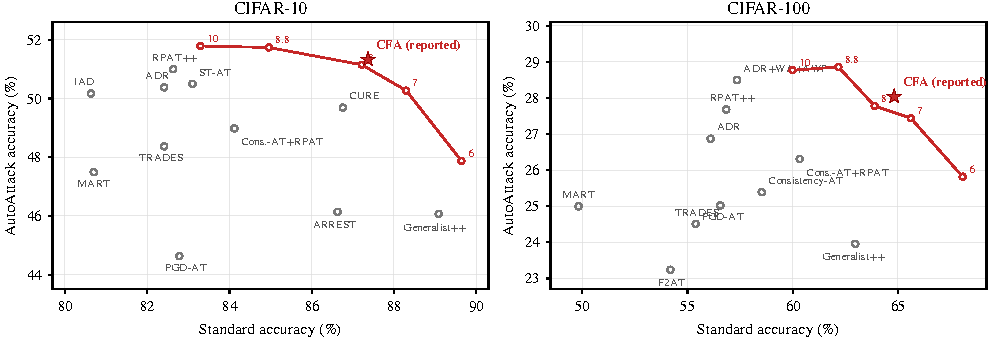
\includegraphics[width=\linewidth]{figure/frontier.pdf}
  \caption{Clean--AutoAttack trade-off on CIFAR-10 and CIFAR-100 with ResNet-18 at
  $\epsilon=8/255$. Grey points
  are published results (\Cref{tab:published}); the CFA curve varies the training radius, and the star
  marks the configuration used elsewhere.}
  \label{fig:frontier}
\end{figure}

Our approach separates the teacher's role as a clean target from the student's response to
perturbations. The teacher supplies a representation at the clean input; the student learns to
preserve it throughout the perturbation set, without matching the teacher at perturbed inputs.
We instantiate this principle as \textbf{Clean Feature Anchoring} (CFA): adversarial training uses
feature regression as the entire backbone objective and retains the teacher's classifier.
Softening probability targets improves robustness in our experiments, but direct regression offers
a competitive alternative without temperature selection. Logit regression is also effective;
the central finding is that clean-target regression can replace, rather than supplement, label supervision.

This single target has a useful structural property. Let $L$ denote the worst-case distance from the
student feature to the clean teacher feature, $F$ the clean teacher--student discrepancy, and $O$ the
diameter of the student's features over the perturbation ball. We show that
$L\le F+O\le3L$. Thus the same objective controls teacher fidelity and local variation without
balancing separate penalties. The result does not certify robust classification, but it explains why
removing the label loss does not leave stability unconstrained.

We further address a mismatch left by a uniform attack radius. The radius is measured in pixels,
whereas CFA measures displacement in feature space, so equal pixel budgets can induce very different
loss changes across examples. Our sensitivity-matched radius assigns less budget to locally sensitive
examples and more to insensitive ones while preserving the batch total. This allocation improves both
axes over the uniform-radius anchor and introduces no additional loss term.

CFA achieves competitive clean--robust trade-offs across CIFAR-10, CIFAR-100, and
Tiny-ImageNet. On CIFAR-100 with ResNet-18 it reaches $62.17\%$ clean and $28.86\%$ AutoAttack
accuracy (\Cref{fig:frontier}). Controlled experiments show that the gain persists without weight
averaging or adversarial weight perturbation, and that substituting label cross-entropy under matched
training conditions reduces both clean and robust accuracy. Varying the natural-teacher checkpoint
reveals that increasing teacher clean accuracy can reduce student clean accuracy while improving
robustness. Changes in the teacher's class separation are also reflected in the student, suggesting
that teacher selection should consider the resulting student trade-off.

Our contributions are threefold:
\begin{itemize}
  \item We show empirically that a natural teacher can supply the sole target for adversarial
  training. CFA realizes this with clean feature regression and an inherited classifier, without
  a label loss or temperature selection during robust training.
  \item We characterize how a fixed anchor controls fidelity and local feature variation, and develop
  a sensitivity-based radius allocation whose benefit persists when the radius distribution is controlled.
  \item Across three datasets and two architectures, we evaluate transfer beyond label training and
  recipe effects, and show that higher teacher clean accuracy need not improve student clean accuracy.
\end{itemize}

\section{Analysis}
\label{sec:analysis}

Adversarial training often improves robustness at the cost of clean accuracy.
To mitigate this trade-off, we explore a self-distillation framework that does not begin with adversarial training, but instead first learns a clean self-teacher exclusively from natural images, thereby preserving a high-accuracy clean representation.
We then transfer the knowledge of this clean self-teacher to the student while adversarially training the student for robustness.
A central question is therefore how the knowledge encoded by the clean self-teacher should be transferred under adversarial perturbations.
We first revisit predictive distillation, where the teacher's softened output distribution serves as the supervision target, as commonly adopted in adversarial distillation.
In contrast, we study direct distillation of the clean self-teacher's feature representation and analyze how a fixed clean feature anchor jointly constrains clean-teacher fidelity and local feature variation.


\subsection{Preliminaries}

Let \(x\in\mathcal X=[0,1]^D\) denote a clean input, and define its \(\ell_\infty\)-bounded perturbation set as
\begin{equation}
B(x,\epsilon)
=
\{x'\in\mathcal X:\lVert x'-x\rVert_\infty\le\epsilon\},
\end{equation}
where \(x'\) denotes a perturbed input within the \(\epsilon\)-neighborhood of \(x\).
During adversarial training, \(x'\) is chosen to maximize the corresponding student loss over \(B(x,\epsilon)\).

We decompose a network as \(f=h\circ\Phi\), where
\(\Phi:\mathcal X\to\mathbb R^d\) is a continuous feature map and
\(h:\mathbb R^d\to\mathbb R^C\), \(h(z)=Wz+b\), is the classifier for \(C\) classes.
We use subscripts \(t\) and \(s\) for the frozen clean self-teacher and the student, respectively.
Both networks share the same architecture, with fixed network statistics for the analysis; feature distances are Euclidean unless stated otherwise.


\subsection{From Soft Predictive Targets to a Fixed Clean Target}
\label{sec:fragile}

Soft-label robust distillation transfers the clean teacher's knowledge through its predictive distribution, typically controlled by a temperature parameter \(\tau\) \citep{ard,rslad,adr,bmtard}.
Given a clean input \(x\) and a perturbed input \(x'\in B(x,\epsilon)\), we define
\begin{equation}
q_t^\tau(x)
=
\operatorname{softmax}(f_t(x)/\tau),
\qquad
p_s^\tau(x')
=
\operatorname{softmax}(f_s(x')/\tau),
\label{eqn:soft_targets}
\end{equation}
where the teacher is evaluated on the clean input \(x\), whereas the student is evaluated on its perturbed counterpart \(x'\).

Conventional knowledge distillation applies the same temperature to both distributions and minimizes the scaled divergence
\begin{equation}
\mathcal L_{\mathrm{KD}}^\tau(x,x')
=
\tau^2
D_{\mathrm{KL}}
\bigl(q_t^\tau(x)\|p_s^\tau(x')\bigr).
\label{eqn:kd_variants}
\end{equation}

Increasing \(\tau\) makes both predictive distributions progressively softer.
In particular, the clean teacher target \(q_t^\tau(x)\) approaches the uniform distribution as \(\tau\to\infty\), and its entropy approaches the maximum value \(\log C\), as illustrated in \Cref{fig:targetcomparison}a.
This does not imply that the shared-temperature KD objective loses all information about the teacher.
Although both distributions become nearly uniform, their deviations from uniformity still encode the relative structure of the underlying logits.

More precisely, for fixed logits and
\[
\bar f
=
f-C^{-1}\mathbf 1\mathbf 1^\top f,
\]
the conventional \(\tau^2\) scaling preserves this residual information in the high-temperature limit:
\begin{equation}
\lim_{\tau\to\infty}
\tau^2
D_{\mathrm{KL}}
\bigl(q_t^\tau(x)\|p_s^\tau(x')\bigr)
=
\frac{1}{2C}
\lVert
\bar f_t(x)-\bar f_s(x')
\rVert_2^2.
\label{eqn:kd_limit}
\end{equation}

Thus, while the softened probabilities themselves approach uniformity, their scaled discrepancy converges to the squared distance between the centered teacher and student logits.
The centering reflects the shift invariance of softmax: adding the same constant to every logit does not change the predictive distribution.
Consequently, high-temperature predictive distillation approaches direct regression of the perturbed student's logits onto the clean self-teacher's logits, up to a common shift.

This connection motivates a more direct view of knowledge transfer.
Rather than passing the clean teacher's knowledge through a softened predictive distribution, we can directly regress the student onto a fixed clean target.
The high-temperature limit naturally gives a logit-level realization of this principle.
CFA instead applies it at the representation level by anchoring the student's perturbed feature to the clean self-teacher feature:
\begin{equation}
\mathcal L_{\mathrm{anchor}}(x)
=
\max_{x'\in B(x,\epsilon)}
\lVert
\Phi_s(x')-\Phi_t(x)
\rVert_2^2.
\label{eqn:anchor_percell}
\end{equation}

Here, \(\Phi_t(x)\) is computed from the clean input and serves as the fixed target, whereas the student is optimized against the worst-case perturbed input within \(B(x,\epsilon)\).
Logit regression constrains the representation through the classifier output, while feature regression directly constrains the representation supplied to the inherited classifier.
We empirically compare these two realizations below.


\begin{figure}[!htbp]
  \centering
  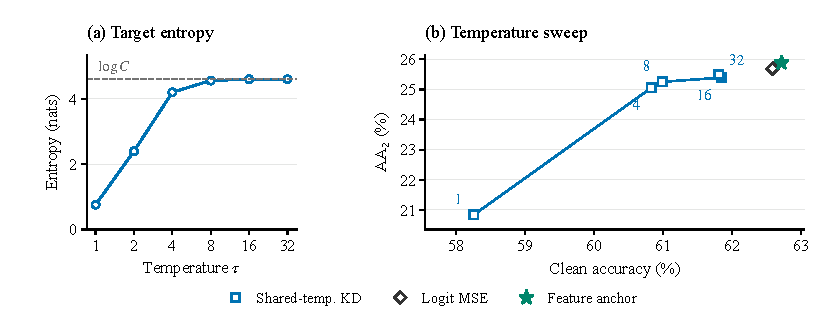
\includegraphics[width=\linewidth]{figure/analysis_targets.pdf}
  \caption{
  Target comparison on CIFAR-100 (ResNet-18).
  (a) Entropy of the clean teacher target \(q_t^\tau(x)\), which approaches the uniform entropy \(\log C\) as the shared temperature \(\tau\) increases.
  (b) Clean accuracy and AA under shared-temperature KD for different values of \(\tau\), together with direct logit and feature regression.
  Numbers denote \(\tau\).
  The full temperature sweep is reported in \Cref{tab:targetcomparison_values}.
  }
  \label{fig:targetcomparison}
\end{figure}


We next compare these forms of supervision to examine how the transition from predictive distillation to direct clean-target regression affects the clean--robust trade-off.
All variants are trained for 50 epochs under an \(\ell_\infty\) perturbation budget of \(\epsilon=8/255\).

As shown in \Cref{fig:targetcomparison}b, increasing the shared temperature moves the KD solution toward the operating point obtained by direct logit regression, consistent with the high-temperature limit in \Cref{eqn:kd_limit}.
This occurs even as the teacher target becomes nearly uniform at large \(\tau\) (\Cref{fig:targetcomparison}a), because the scaled discrepancy retains the relative structure of the underlying logits.

Direct feature regression yields \(0.13\) and \(0.19\) percentage-point improvements in clean accuracy and AA, respectively, over logit regression.
Under the final training recipe, the corresponding differences remain small at \(0.26/0.13\) points (\Cref{tab:finalallocation}).
Thus, direct regression onto a fixed clean target provides a temperature-free alternative to predictive distillation, while the small gap between logit and feature regression does not by itself establish an inherent empirical advantage of feature coordinates.

We also note that KD updates the classifier, whereas the regression variants keep it fixed.
The comparison therefore evaluates complete training designs rather than isolating the target representation alone.

\label{sec:sole_target}

The comparison shifts our focus from how a predictive distribution should be softened to what is controlled by anchoring the student to a fixed clean target.
We next characterize this fixed-anchor property for the feature-space realization used by CFA.


\subsection{What the Anchor Controls}
\label{sec:decomp}

CFA is designed to preserve the representation of the clean self-teacher while the student is trained against adversarial perturbations.
We therefore ask what controlling the fixed-anchor objective implies about the student's representation.
In particular, a desirable student should remain faithful to the clean teacher at the original input while exhibiting limited feature variation within the perturbation set.

To formalize these properties, let \(x\in\mathcal X\) and \(B=B(x,\epsilon)\), and define
\begin{equation}
L
=
\max_{x'\in B}
\lVert\Phi_s(x')-\Phi_t(x)\rVert_2,
\qquad
F
=
\lVert\Phi_s(x)-\Phi_t(x)\rVert_2,
\qquad
O
=
\max_{x',x''\in B}
\lVert\Phi_s(x')-\Phi_s(x'')\rVert_2.
\label{eqn:LFO}
\end{equation}

Here, \(L\) is the worst-case discrepancy from the fixed clean teacher anchor and corresponds to the quantity directly controlled by the CFA objective.
\(F\) measures the clean feature discrepancy between the student and its self-teacher, capturing the fidelity of the transferred clean representation.
\(O\) measures the diameter of the student's feature set over the perturbation region and thus its local feature variation.

These quantities satisfy the following relation.

\begin{proposition}[Fixed-anchor decomposition]
\label{prop:decomp}
For every \(x\in\mathcal X\) and \(\epsilon\ge0\),
\begin{equation}
L
\le
F+O
\le
3L.
\label{eqn:decomp}
\end{equation}
\end{proposition}

\begin{proof}
For any \(x'\in B\), the triangle inequality gives
\[
\lVert\Phi_s(x')-\Phi_t(x)\rVert_2
\le
\lVert\Phi_s(x')-\Phi_s(x)\rVert_2
+
\lVert\Phi_s(x)-\Phi_t(x)\rVert_2
\le
O+F.
\]
Maximizing over \(x'\in B\) yields \(L\le F+O\).

Conversely, since \(x\in B\),
\[
F
=
\lVert\Phi_s(x)-\Phi_t(x)\rVert_2
\le L.
\]
Moreover, for any \(x',x''\in B\),
\[
\begin{aligned}
\lVert\Phi_s(x')-\Phi_s(x'')\rVert_2
&\le
\lVert\Phi_s(x')-\Phi_t(x)\rVert_2
+
\lVert\Phi_s(x'')-\Phi_t(x)\rVert_2 \\
&\le
2L.
\end{aligned}
\]
Hence \(O\le2L\), and therefore \(F+O\le3L\).
\end{proof}

The proposition gives a direct interpretation of the CFA objective.
If \(L\le\delta\), then
\[
F\le\delta,
\qquad
O\le2\delta.
\]
Thus, keeping the worst-case student feature close to the clean teacher anchor simultaneously keeps the student's clean representation close to the teacher and limits feature variation throughout the perturbation region.
Importantly, this conclusion does not require the clean teacher itself to be robust or locally stable; only its representation at the clean input \(\Phi_t(x)\) serves as the anchor.

Because CFA inherits the teacher's linear classifier, the same discrepancy also bounds the deviation at the classifier output.
For \(h_t(z)=W_tz+b_t\),
\begin{equation}
\lVert
h_t(\Phi_s(x'))
-
h_t(\Phi_t(x))
\rVert_2
\le
\lVert W_t\rVert_{2\rightarrow2}
\lVert
\Phi_s(x')-\Phi_t(x)
\rVert_2
\le
\lVert W_t\rVert_{2\rightarrow2}L.
\end{equation}
A small anchor discrepancy therefore limits how far the student's logits can deviate from the clean teacher logits under the inherited classifier.
This bound alone does not guarantee identical predictions, which additionally depend on the teacher's clean classification margin.

The fixed-anchor argument is not specific to feature coordinates and analogously applies to norm-based regression onto a fixed logit target.
It therefore characterizes the joint control induced by a fixed target rather than establishing an inherent advantage of feature matching.
In practice, finite-step PGD only approximates the inner maximization and thus does not certify the true value of \(L\).

\FloatBarrier


\subsection{How Does Teacher Performance Affect Transfer?}
\label{sec:teacher_transfer}
\label{sec:geometry}

The preceding analysis shows that anchoring the student to a fixed clean target can preserve its agreement with the self-teacher while limiting local feature variation.
This raises a natural question about the teacher itself: does a better-performing clean self-teacher necessarily provide a better target for robust transfer?

A straightforward expectation is that a teacher with higher clean accuracy should provide stronger clean supervision and consequently yield a better student.
We first examine this hypothesis using different checkpoints along the training trajectory of the same clean self-teacher.
Because each checkpoint determines the student's initialization, feature target, and inherited classifier, this experiment measures the combined effect of the teacher state transferred to the student.


\begin{figure}[!htbp]
  \centering
  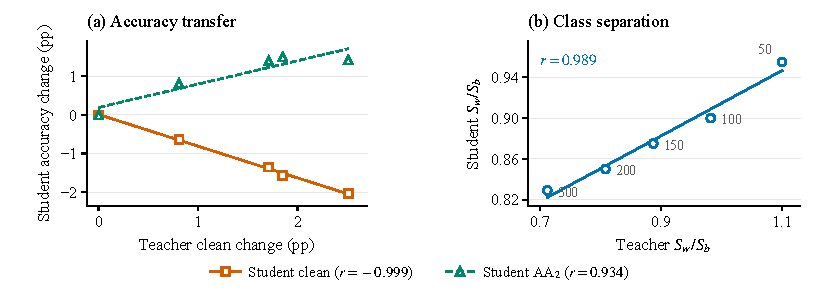
\includegraphics[width=\linewidth]{figure/teacher_checkpoint_trends.pdf}
  \caption{
  Transfer from clean self-teachers at different stages of training on CIFAR-100 (ResNet-18).
  (a) Changes in teacher clean accuracy and resulting student clean accuracy and AA relative to the 50-epoch teacher.
  (b) Within-to-between scatter ratios \(S_w/S_b\) of teacher and student features; lower values indicate stronger class separation, and labels denote teacher epochs.
  Lines are least-squares fits.
  Exact values are reported in \Cref{tab:teacherladder_values}.
  }
  \label{fig:teacherladder}
\end{figure}


As the clean self-teacher is trained from 50 to 300 epochs, its clean accuracy increases by \(2.51\) percentage points.
This improvement, however, does not translate into a simultaneous improvement in the student's clean and robust performance.
Student clean accuracy decreases by \(2.04\) points, while AA increases from \(24.38\%\) to \(25.80\%\) (\Cref{fig:teacherladder}a).
Thus, increasing teacher clean accuracy shifts the student's clean--robust operating point rather than uniformly improving it.
The trend is also not strictly monotonic: the student transferred from the 200-epoch teacher achieves slightly higher AA than that transferred from the 300-epoch teacher.

To examine whether this behavior is specific to a single teacher trajectory, we repeat the experiment with an independently trained clean self-teacher.
The same overall pattern emerges.
From 40 to 300 teacher epochs, teacher clean accuracy increases from \(75.57\%\) to \(78.27\%\), whereas student clean accuracy decreases from \(64.36\%\) to \(62.34\%\) and AA increases from \(23.86\%\) to \(25.94\%\) (\Cref{tab:teachertrajectory}).
Across both trajectories, higher teacher clean accuracy therefore accompanies a shift in the student's clean--robust trade-off rather than a uniform improvement in student performance.


\begin{table}[!htbp]
  \centering
  \small
  \setlength{\tabcolsep}{6pt}
  \caption{
  Transfer from an independently trained clean self-teacher trajectory on CIFAR-100 (ResNet-18; 50-epoch students).
  Full results are reported in \Cref{tab:teacherladder_seed1}.
  }
  \label{tab:teachertrajectory}
  \begin{tabular}{rrrrr}
    \toprule
    Teacher epoch & Teacher clean & Student clean & Student AA & Student NRR \\
    \midrule
    40  & 75.57 & 64.36 & 23.86 & 34.81 \\
    100 & 77.27 & 63.68 & 25.61 & 36.53 \\
    200 & 77.90 & 63.02 & 26.16 & 36.97 \\
    300 & 78.27 & 62.34 & 25.94 & 36.64 \\
    \bottomrule
  \end{tabular}
\end{table}


Teacher clean accuracy alone does not reveal what changes in the transferred representation as training progresses.
To examine the representation associated with this shift, we measure the within-to-between scatter ratio \(S_w/S_b\) on unit-normalized clean features.
As shown in \Cref{fig:teacherladder}b, the teacher and student ratios decrease together as teacher training progresses, indicating increasingly separated class structure in both representations.
This association suggests that changes in the teacher representation are reflected in the resulting student, but does not identify which representational property causes the observed clean--robust shift.

The checkpoint comparison couples teacher accuracy with training stage and other changes in the learned representation.
We therefore further ask whether clean accuracy alone is sufficient to characterize a teacher for transfer.
To separate teacher accuracy from training stage, we compare clean self-teachers trained with label smoothing and mixup that achieve nearly identical clean accuracy.


\begin{table}[!htbp]
  \centering
  \small
  \setlength{\tabcolsep}{4.5pt}
  \caption{
  Transfer from accuracy-matched clean self-teachers on CIFAR-100 (ResNet-18; 50-epoch students).
  Feature sensitivity is measured on held-out data.
  }
  \label{tab:matchedteacher}
  \begin{tabular}{lrrcrr}
    \toprule
    & \multicolumn{2}{c}{Teacher} && \multicolumn{2}{c}{Student} \\
    \cmidrule(lr){2-3}\cmidrule(lr){5-6}
    Natural training & Clean & Sensitivity && Clean & AA \\
    \midrule
    Label smoothing \(0.1\) & 78.76 & 3.16 && 59.62 & 25.72 \\
    Mixup                 & 78.62 & 4.82 && 63.80 & 25.70 \\
    \bottomrule
  \end{tabular}
\end{table}


Despite differing by only \(0.14\) percentage points in teacher clean accuracy, the two teachers produce students whose clean accuracies differ by \(4.18\) points, while their AA differs by only \(0.02\) points (\Cref{tab:matchedteacher}).
Teacher clean accuracy is therefore insufficient to characterize how the clean representation will transfer to the adversarially trained student.
The teachers also differ in feature sensitivity in the same order as student clean accuracy, suggesting that properties of the transferred representation beyond teacher accuracy may be relevant.
With only one accuracy-matched pair, however, this observation is insufficient to establish feature sensitivity as a general predictor of transfer.

Taken together, these results show that the role of the clean self-teacher cannot be summarized by its clean accuracy alone.
As the teacher representation evolves, the resulting student can move to a different point on the clean--robust trade-off even as teacher clean accuracy improves, and teachers with nearly matched clean accuracy can transfer differently.
We use the 200-epoch clean self-teacher for the subsequent experiments and next consider a source of variation that remains after the teacher is fixed: the same perturbation radius need not induce the same anchor discrepancy across individual examples.
\section{Method}
\label{sec:method}

\subsection{Clean Feature Anchoring}
\label{sec:anchor}

Let $\Phi_t$ and $h_t$ be the frozen feature map and classifier of the natural teacher. The student
inherits both, $\Phi_s\leftarrow\Phi_t$ and $h_s=h_t$, after which only $\Phi_s$ is optimized. For a
clean example $x$, CFA solves
\begin{equation}
\begin{aligned}
x_{\mathrm{adv}}
&=\operatorname*{arg\,max}_{x'\in B(x,\epsilon)}
  \lVert\Phi_s(x')-\Phi_t(x)\rVert_2^2,\\
\mathcal L_{\mathrm{CFA}}
&=\mathbb E_x\!\left[\lVert\Phi_s(x_{\mathrm{adv}})-\Phi_t(x)\rVert_2^2\right].
\end{aligned}
\label{eqn:anchor}
\end{equation}
We approximate the inner maximization with randomly initialized PGD against the fixed target
$\Phi_t(x)$ and minimize the same discrepancy over the backbone. This adversarial-training stage
uses no label loss; inference uses $h_t\circ\Phi_s$. \Cref{alg:cfa} gives the complete procedure.

\subsection{Sensitivity-Matched $\epsilon$}
\label{sec:angeps}

A uniform pixel radius need not produce a uniform change in the feature-space objective. We therefore
allocate the batch budget according to each example's clean-point loss sensitivity. For
$\ell_{\mathrm{anc}}(x';x_i)=\lVert\Phi_s(x')-\Phi_t(x_i)\rVert_2^2$, define
\begin{equation}
g_i=\left.\lVert\nabla_{x'}\ell_{\mathrm{anc}}(x';x_i)\rVert_1\right|_{x'=x_i},
\qquad
\max_{\lVert\delta\rVert_\infty\le e}
\langle\nabla_{x'}\ell_{\mathrm{anc}},\delta\rangle=e g_i.
\label{eqn:firstorder}
\end{equation}
The linearized loss change under radius $\epsilon_i$ is therefore $\epsilon_i g_i$. For $g_i>0$,
equalizing this quantity while preserving $\sum_i\epsilon_i=N\epsilon$ gives
\begin{equation}
\epsilon_i=N\epsilon\frac{g_i^{-1}}{\sum_jg_j^{-1}},
\qquad\text{or more generally}\qquad
\epsilon_i\propto g_i^{-p},
\label{eqn:angeps_ideal}
\end{equation}
where $p=0$ recovers a uniform radius. We use $p=1$ and an $\ell_2$ gradient norm as a sensitivity
proxy, measured with one backward pass at clean inputs. The $\ell_1$ version implied by
\Cref{eqn:firstorder} gives $0.29$ points lower AA and retains the clean-accuracy gain
(\Cref{app:box}); exact first-order equalization is therefore a motivation for the implemented rule.

We floor the proxy at $10^{-12}$, clip its inverse-mean multipliers to $[0.5,1.5]$, and normalize
them to unit mean before setting $\epsilon_i$. The floor gives a uniform allocation when all clean
gradients vanish at teacher initialization. Normalization preserves $\sum_i\epsilon_i=N\epsilon$,
although the final multipliers can leave the clipping interval. PGD step sizes are scaled by the same
multipliers. \Cref{app:box} specifies this procedure and an optional exact-box variant.
The matched-budget comparison in \Cref{tab:allocation} tests whether the sensitivity signal improves
on uniform, difficulty-based, and margin-based allocation.

\section{Experiments}
\label{sec:exp}

We evaluate CFA with three questions in mind: how it compares with existing
adversarial training and robust distillation methods, whether its performance
generalizes across datasets and model architectures, and how its individual
design components contribute to the resulting clean--robust trade-off.


\subsection{Experimental Settings}

We evaluate CFA on CIFAR-10, CIFAR-100
\citep{krizhevsky2009learning}, and Tiny-ImageNet-200
\citep{le2015tiny}, using ResNet-18 as the default architecture.
We additionally evaluate WideResNet-34-10 to examine generalization across
model capacity.

Unless stated otherwise, the clean self-teacher is trained on natural images
for 200 epochs and then frozen. The student is initialized from the teacher,
with the inherited classifier kept fixed during adversarial training.
Following \Cref{sec:method}, the student is trained using clean feature
anchoring with sensitivity-matched perturbation radii (\(p=1\)).
The main CIFAR experiments use 150 training epochs and
\(\epsilon_{\mathrm{train}}=8/255\).
We use AdamW with a one-cycle learning-rate schedule and 10-step PGD,
together with weight averaging (WA) and adversarial weight perturbation
(AWP). Teacher statistics and dataset- and architecture-specific training
settings are reported in \Cref{tab:teachers,app:repro}.

We compare CFA with standard adversarial training and robust distillation
baselines using their respective training recipes. Distillation-based
baselines receive the same clean self-teacher where applicable.
We report clean accuracy and AutoAttack (AA) accuracy on the full test set at
\(\epsilon=8/255\), together with their arithmetic mean (Avg) and harmonic
mean (NRR). Additional evaluation details, attack diagnostics, and results
with alternative teachers are provided in
\Cref{app:repro,app:gradmask,tab:published}.


\subsection{Main Results}

\begin{table}[!htbp]
  \centering
  \footnotesize
  \setlength{\tabcolsep}{3.2pt}
  \caption{
  ResNet-18 results under \(\ell_\infty\) perturbations with
  \(\epsilon=8/255\). All values are measured in our framework.
  \emph{T.} denotes the teacher assumed by each method: none (--),
  a natural model (nat.), or the method's own weight average (self).
  The CIFAR-100 CFA row reports the mean of three student seeds;
  all other rows are individual runs.
  }
  \label{tab:main}
  \begin{tabular}{llrrrrrrrr}
    \toprule
    & & \multicolumn{4}{c}{CIFAR-10}
      & \multicolumn{4}{c}{CIFAR-100} \\
    \cmidrule(lr){3-6}\cmidrule(lr){7-10}
    Method & T. & Clean & AA & Avg & NRR
           & Clean & AA & Avg & NRR \\
    \midrule
    PGD-AT & -- & 84.54 & 43.57 & 64.06 & 57.50
                 & 57.36 & 20.34 & 38.85 & 30.03 \\
    TRADES & -- & 81.71 & 49.16 & 65.44 & 61.39
                 & 55.28 & 23.55 & 39.42 & 33.03 \\
    MART   & -- & 80.41 & 45.56 & 62.99 & 58.16
                 & 53.86 & 22.72 & 38.29 & 31.96 \\
    \midrule
    ARD & nat. & 84.58 & 43.75 & 64.16 & 57.67
               & 57.61 & 20.24 & 38.93 & 29.96 \\
    RSLAD & nat. & 85.15 & 42.91 & 64.03 & 57.06
                 & 59.68 & 21.30 & 40.49 & 31.40 \\
    AdaAD & nat. & 85.39 & 46.22 & 65.81 & 59.98
                 & 59.79 & 23.19 & 41.49 & 33.42 \\
    AdaAD + IGDM & nat. & 85.01 & 45.50 & 65.26 & 59.27
                        & 48.25 & 19.48 & 33.87 & 27.75 \\
    LBGAT & nat. & -- & -- & -- & --
                 & 56.46 & 26.02 & 41.24 & 35.62 \\
    ARREST & nat. & 85.06 & 46.42 & 65.74 & 60.06
                  & \textbf{66.97} & 22.78 & 44.88 & 34.00 \\
    \midrule
    HAT & nat. & 84.59 & 48.81 & 66.70 & 61.90
               & 60.67 & 24.45 & 42.56 & 34.85 \\
    ADR & self & 83.36 & 49.72 & 66.54 & 62.29
               & 59.93 & 27.20 & 43.57 & 37.42 \\
    RPAT++ & -- & 82.41 & 50.75 & 66.58 & 62.82
                  & 55.93 & 27.36 & 41.64 & 36.74 \\
    \midrule
    \textbf{CFA (ours)}
      & nat.
      & \textbf{87.37} & \textbf{51.33}
      & \textbf{69.35} & \textbf{64.67}
      & \textbf{64.82} & \textbf{28.04}
      & \textbf{46.43} & \textbf{39.15} \\
    \bottomrule
  \end{tabular}
\end{table}

\Cref{tab:main} compares CFA with standard adversarial training and robust
distillation methods on CIFAR-10 and CIFAR-100.
On CIFAR-100, CFA achieves \(64.82\%\) clean accuracy and \(28.04\%\) AA,
yielding an NRR of \(39.15\).
Compared with ADR, the closest baseline in NRR, CFA improves clean accuracy
by \(4.89\) points, AA by \(0.84\) points, and NRR by \(1.73\) points.
ARREST achieves higher clean accuracy at \(66.97\%\), but its AA is
\(5.26\) points lower than CFA, reflecting a different clean--robust
operating point.

On CIFAR-10, CFA reaches \(87.37\%\) clean accuracy and \(51.33\%\) AA,
with an NRR of \(64.67\).
Its NRR exceeds the closest baseline by \(1.85\) points.
Together, these results show that CFA maintains high clean accuracy while
remaining competitive in robust accuracy across both CIFAR datasets.


\subsection{Generalization Across Datasets and Architectures}

We next examine whether the behavior observed on the CIFAR benchmarks
extends to a larger-scale dataset and a higher-capacity architecture.

\begin{table}[!htbp]
  \centering
  \footnotesize
  \setlength{\tabcolsep}{3.2pt}
  \caption{
  Results on Tiny-ImageNet-200 with ResNet-18 and CIFAR-10 with
  WideResNet-34-10, measured in our framework.
  }
  \label{tab:scale}
  \begin{tabular}{llrrrrrrrr}
    \toprule
    & & \multicolumn{4}{c}{Tiny-ImageNet, ResNet-18}
      & \multicolumn{4}{c}{CIFAR-10, WRN-34-10} \\
    \cmidrule(lr){3-6}\cmidrule(lr){7-10}
    Method & T. & Clean & AA & Avg & NRR
           & Clean & AA & Avg & NRR \\
    \midrule
    PGD-AT & -- & 49.72 & 14.45 & 32.09 & 22.39
                 & 86.00 & 45.71 & 65.86 & 59.69 \\
    TRADES & -- & 46.98 & 15.95 & 31.46 & 23.83
                 & 85.13 & 48.99 & 67.06 & 62.19 \\
    MART & -- & 46.01 & 16.90 & 31.46 & 24.73
               & 85.29 & 47.06 & 66.18 & 60.65 \\
    \midrule
    ARD & nat. & 49.74 & 14.48 & 32.11 & 22.43
               & 86.35 & 45.52 & 65.94 & 59.61 \\
    RSLAD & nat. & 51.26 & 17.02 & 34.14 & 25.56
                 & 86.41 & 45.80 & 66.10 & 59.87 \\
    AdaAD & nat. & 51.59 & 16.79 & 34.19 & 25.33
                 & 86.80 & 46.84 & 66.82 & 60.85 \\
    LBGAT & nat. & 51.04 & 18.47 & 34.75 & 27.13
                 & 81.56 & 51.79 & 66.68 & 63.35 \\
    ARREST & nat. & \textbf{59.38} & 16.06 & 37.72 & 25.28
                  & 87.54 & 48.83 & 68.19 & 62.69 \\
    HAT & nat. & 52.57 & 17.28 & 34.93 & 26.01
               & 87.15 & 53.21 & 70.18 & 66.07 \\
    ADR & self & 47.66 & \textbf{20.85} & 34.25 & 29.01
               & 88.64 & 52.34 & 70.49 & 65.82 \\
    \midrule
    \textbf{CFA (ours)}
      & nat.
      & 55.16 & 20.54 & \textbf{37.85} & \textbf{29.93}
      & \textbf{88.67} & \textbf{55.29}
      & \textbf{71.98} & \textbf{68.11} \\
    \bottomrule
  \end{tabular}
\end{table}

On Tiny-ImageNet-200, CFA achieves the highest Avg and NRR without maximizing
either endpoint individually (\Cref{tab:scale}).
ARREST attains higher clean accuracy, while ADR exceeds CFA in AA by
\(0.31\) points.
CFA instead reaches \(55.16\%\) clean accuracy and \(20.54\%\) AA,
resulting in the highest NRR of \(29.93\).

The effect of the clean self-teacher observed in
\Cref{sec:teacher_transfer} is also present on Tiny-ImageNet.
Replacing the 200-epoch reference teacher with an 80-epoch teacher changes
the resulting student from \(55.16/20.54\) to \(57.08/18.96\)
clean/AA.
This again illustrates that changing the clean teacher can shift the
student's clean--robust operating point rather than uniformly improving both
metrics.

With WideResNet-34-10 on CIFAR-10, CFA achieves \(88.67\%\) clean accuracy
and \(55.29\%\) AA.
Its clean accuracy is nearly identical to ADR
(\(88.64\%\)), while its AA is \(2.95\) points higher.
On CIFAR-100 with the same architecture, CFA reaches
\(65.04/30.14\) clean/AA, compared with \(64.50/29.04\) for ADR
(\Cref{tab:wrn100}).
These results indicate that the observed behavior is not restricted to
ResNet-18 or to a single dataset.


\subsection{Ablation and Component Analysis}
\label{sec:components}

We next examine the components underlying CFA.
We first isolate the clean feature-anchoring objective, then compare feature
and logit targets, and finally study the contribution and assignment of
sample-dependent perturbation radii.
We separately report the effects of weight averaging and AWP.


\paragraph{Clean feature anchoring.}

We first test whether the gain arises from the clean feature anchor rather
than from the surrounding adversarial-training recipe.
Under the same base training regime, replacing feature anchoring with
label-based cross-entropy reduces both clean and robust accuracy.

\begin{table}[!htbp]
  \centering
  \small
  \setlength{\tabcolsep}{5pt}
  \caption{
  Objective control on CIFAR-100 with ResNet-18, 100 epochs, no weight
  averaging or AWP, \(p=0\), and
  \(\epsilon_{\mathrm{train}}=8.8/255\).
  }
  \label{tab:controls}
  \begin{tabular}{lrrr}
    \toprule
    Objective & Clean & AA & NRR \\
    \midrule
    Anchor
      & \textbf{61.29} & \textbf{25.36} & \textbf{35.88} \\
    Label cross-entropy, same recipe
      & 54.60 & 19.45 & 28.68 \\
    Label cross-entropy, own recipe
      & 56.66 & 20.91 & 30.55 \\
    \bottomrule
  \end{tabular}
\end{table}

As shown in \Cref{tab:controls}, replacing the anchor objective with
cross-entropy under the same recipe reduces clean accuracy by \(6.69\)
points and AA by \(5.91\) points.
Allowing cross-entropy to use its own optimizer and schedule narrows the gap,
but CFA remains ahead by \(4.63\) clean and \(4.45\) AA points.
Initialization and schedule controls change NRR by at most \(0.22\)
(\Cref{tab:recipe}), indicating that the difference cannot be attributed
solely to these training choices.


\paragraph{Feature and logit targets.}

The analysis in \Cref{sec:fragile} showed that fixed-target regression need
not be restricted to feature coordinates.
We therefore compare feature anchoring with direct logit regression under
otherwise comparable training conditions.

At a uniform radius of \(8.8/255\) and 100 training epochs, logit regression
reaches \(60.36/28.02\) clean/AA, compared with \(60.42/28.42\) for
feature regression (\Cref{tab:regression_stack}).
Under the final 150-epoch recipe with sensitivity-matched radii, logit
regression reaches \(64.49/27.85\) clean/AA (NRR \(38.90\)), compared with
\(64.82/28.04\) (NRR \(39.15\)) for feature regression
(\Cref{tab:finalallocation}).
The small differences are consistent with our analysis: effective transfer
through a fixed clean target is not confined to feature space.


\paragraph{Sensitivity-matched radius allocation.}

We next isolate the second component of CFA: allocating the perturbation
radius according to local sensitivity.
We hold the teacher, training schedule, mean radius, weight averaging, and
AWP fixed and vary only the radius allocation.

\begin{table}[!htbp]
  \centering
  \small
  \setlength{\tabcolsep}{5pt}
  \caption{
  Clean-target regression in the final CIFAR-100 recipe
  (ResNet-18, 150 epochs, \(\epsilon_{\mathrm{train}}=8/255\)).
  Feature rows report mean \(\pm\) sample standard deviation over three
  student seeds and differ only in \(p\); logit regression is one run at
  \(p=1\).
  }
  \label{tab:finalallocation}
  \begin{tabular}{lrrr}
    \toprule
    Target and radius & Clean & AA & NRR \\
    \midrule
    Features, uniform (\(p=0\))
      & \(62.63\pm0.22\)
      & \(28.01\pm0.20\)
      & \(38.71\pm0.21\) \\
    Features, sensitivity-matched (\(p=1\))
      & \(\mathbf{64.82\pm0.07}\)
      & \(\mathbf{28.04\pm0.09}\)
      & \(\mathbf{39.15\pm0.09}\) \\
    Logits, sensitivity-matched (\(p=1\))
      & 64.49 & 27.85 & 38.90 \\
    \bottomrule
  \end{tabular}
\end{table}

Replacing the uniform radius with sensitivity matching increases clean
accuracy by \(2.19\pm0.20\) points across three paired runs, while AA changes
by only \(0.03\pm0.23\) points (\Cref{tab:finalallocation}).
The clean-accuracy improvement appears in every seed, whereas the AA
difference is comparable to run-to-run variation.
Thus, in the final training configuration, sensitivity matching primarily
shifts the operating point toward higher clean accuracy without an observed
loss in AA.
This empirical behavior is not implied by the first-order motivation in
\Cref{sec:angeps}, which only motivates how the perturbation budget is
allocated.


\paragraph{Which signal should allocate the radius?}

The previous comparison establishes the effect of sensitivity matching
relative to a uniform radius, but does not determine whether the sensitivity
signal itself matters or whether heterogeneous radii are sufficient.
We therefore compare sensitivity with alternative assignments under the same
mean perturbation budget.

\begin{table}[!htbp]
  \centering
  \small
  \setlength{\tabcolsep}{4.5pt}
  \caption{
  Radius-allocation signals under the same mean radius on CIFAR-100 with
  ResNet-18, trained for 100 epochs with WA and AWP.
  \(\mathrm{sd}(w)\) measures multiplier dispersion.
  }
  \label{tab:allocation}
  \begin{tabular}{lrrrr}
    \toprule
    Allocation & \(\mathrm{sd}(w)\) & Clean & AA & NRR \\
    \midrule
    Uniform
      & 0 & 60.42 & 28.42 & 38.66 \\
    Sensitivity
      & 0.32 & \textbf{62.17} & \textbf{28.86} & \textbf{39.42} \\
    Same multipliers, difficulty order
      & 0.32 & 60.90 & 28.06 & 38.42 \\
    Difficulty magnitude
      & 0.39 & 61.27 & 28.12 & 38.55 \\
    Logit margin
      & 0.42 & 61.07 & 27.79 & 38.20 \\
    \bottomrule
  \end{tabular}
\end{table}

Sensitivity matching gives the highest clean accuracy, AA, and NRR among the
tested allocation signals (\Cref{tab:allocation}).
In particular, reassigning the same set of sensitivity-derived radius
multipliers according to sample difficulty reduces AA by \(0.80\) points and
NRR from \(39.42\) to \(38.42\).
Because this control preserves the radius distribution while changing which
example receives each radius, the result indicates that the gain cannot be
explained solely by introducing heterogeneous perturbation radii.
Difficulty magnitude and logit-margin allocation also yield lower NRR than
the sensitivity-based assignment.


\paragraph{Weight averaging and AWP.}

Finally, we examine the additional training components used in the final
configuration.
Weight averaging and AWP are not defining components of the CFA objective,
but are included in the final recipe to strengthen adversarial training.
In the ordered ablation, adding weight averaging and AWP increases AA by
\(1.95\) and \(1.17\) points, respectively
(\Cref{tab:ladder}).
Because this ordered ablation does not isolate interactions between the two
components, additional radius and training-stack comparisons are reported in
\Cref{tab:radius,tab:stackboth}.

To verify that the final training stack alone does not account for CFA's
performance, we also apply teacher initialization, weight averaging, and AWP
to the baseline methods.

\begin{table}[!htbp]
  \centering
  \scriptsize
  \setlength{\tabcolsep}{4pt}
  \caption{
  Adding teacher initialization, weight averaging, and AWP to baseline
  recipes on CIFAR-100 (ResNet-18).
  }
  \label{tab:baselinestack}
  \begin{tabular}{lrrrcrrr}
    \toprule
    & \multicolumn{3}{c}{Own recipe}
    && \multicolumn{3}{c}{+ teacher init + WA + AWP} \\
    \cmidrule(lr){2-4}\cmidrule(lr){6-8}
    Method & Clean & AA & NRR && Clean & AA & NRR \\
    \midrule
    PGD-AT & 57.36 & 20.34 & 30.03
           && 59.85 & 25.77 & 36.03 \\
    TRADES & 55.28 & 23.55 & 33.03
           && 56.16 & 24.56 & 34.17 \\
    MART & 53.86 & 22.72 & 31.96
         && 50.97 & 25.13 & 33.66 \\
    ARD & 57.61 & 20.24 & 29.96
        && 60.19 & 26.10 & 36.41 \\
    RSLAD & 59.68 & 21.30 & 31.40
          && 63.44 & 25.55 & 36.43 \\
    AdaAD & 59.79 & 23.19 & 33.42
          && 57.21 & 27.10 & 36.78 \\
    AdaAD + IGDM & 48.25 & 19.48 & 27.75
                 && 54.24 & 25.56 & 34.75 \\
    Consistency-AT & 57.53 & 20.01 & 29.69
                   && 60.74 & 25.38 & 35.80 \\
    LBGAT & 56.46 & 26.02 & 35.62
          && 53.91 & 25.16 & 34.31 \\
    ADR & 59.93 & 27.20 & 37.42
        && 59.84 & 27.84 & 38.00 \\
    HAT & 60.67 & 24.45 & 34.85
        && 57.63 & 24.74 & 34.62 \\
    ARREST & 66.44 & 22.99 & 34.16
           && 64.95 & 23.02 & 33.99 \\
    \midrule
    \textbf{CFA (ours)}
      & \multicolumn{3}{c}{---}
      && \textbf{64.82} & \textbf{28.04} & \textbf{39.15} \\
    \bottomrule
  \end{tabular}
\end{table}

The additional training components increase NRR for nine of the twelve
baselines, but none reaches CFA's NRR of \(39.15\)
(\Cref{tab:baselinestack}); ADR is the closest at \(38.00\).
This comparison indicates that the performance of CFA cannot be attributed
solely to teacher initialization, weight averaging, or AWP.
ARREST uses its 20-epoch recipe in this control, whereas
\Cref{tab:main} reports its 150-epoch comparison; ADR already includes a
SAM-style weight perturbation in its original recipe.

Attack diagnostics, repeat-seed results, and additional implementation
controls are provided in \Cref{app:gradmask,app:repro}.
\appendix

\section{Algorithm}
\label{app:alg}

\begin{algorithm}[h]
\caption{Clean Feature Anchoring (CFA)}
\label{alg:cfa}
\begin{algorithmic}[1]
\STATE {\bfseries Input:} dataset $\mathcal{D}$, radius $\epsilon$, attack steps $K$, step size $a$,
  exponent $p$, clipping thresholds $[w_{\mathrm{lo}}, w_{\mathrm{hi}}]$
\STATE {\bfseries Output:} robust student $h_t \circ \Phi_s$
\STATE
\STATE \COMMENT{\emph{Phase 1 --- natural self-teacher.} The only stage that uses labels.}
\STATE Train $f_t = h_t \circ \Phi_t$ on $\mathcal{D}$ with standard cross-entropy; freeze it
\STATE
\STATE \COMMENT{\emph{Phase 2 --- anchored adversarial training.} No labels, no head update.}
\STATE $\Phi_s \leftarrow \Phi_t$ \hfill \COMMENT{student initialized at the teacher}
\FOR{$\mathrm{epoch} = 1$ {\bfseries to} $T$}
  \FOR{minibatch $\{x_i\}_{i=1}^{N} \subset \mathcal{D}$}
    \STATE $\phi_i \leftarrow \Phi_t(x_i)$ \hfill \COMMENT{teacher read once, at the clean input}
    \STATE $g_i \leftarrow \max(\lVert \nabla_x \lVert \Phi_s(x_i) - \phi_i \rVert^2 \rVert_2,10^{-12})$
      \hfill \COMMENT{one backward pass}
    \STATE $v_i \leftarrow \mathrm{clip}((\bar g/g_i)^p,w_{\mathrm{lo}},w_{\mathrm{hi}})$;
      $w_i \leftarrow Nv_i/\sum_jv_j$
    \STATE $\epsilon_i \leftarrow \epsilon w_i$; $a_i\leftarrow a w_i$
      \hfill \COMMENT{$\textstyle\sum_i \epsilon_i = N\epsilon$}
    \STATE $x_i^{0} \leftarrow x_i + \eta_i$
    \FOR{$k = 0$ {\bfseries to} $K-1$}
      \STATE $x_i^{k+1} \leftarrow \Pi_{B(x_i, \epsilon_i)}
        \big( x_i^{k} + a_i\,\mathrm{sign}\,\nabla_x \lVert \Phi_s(x_i^{k}) - \phi_i \rVert^2 \big)$
    \ENDFOR
    \STATE $\mathcal{L} \leftarrow \frac{1}{N} \sum_i
      \lVert \Phi_s(x_i^{K}) - \phi_i \rVert^2$
    \STATE $\Phi_s \leftarrow \Phi_s - \mu \nabla_{\Phi_s} \mathcal{L}$
      \hfill \COMMENT{$h_t$ is never updated}
  \ENDFOR
\ENDFOR
\end{algorithmic}
\end{algorithm}

\section{Two Partial Results on the Robustness Side}
\label{app:robustness}

Natural-teacher guidance is shared with prior work; our question is whether a fixed clean target can
support adversarial training without an additional label objective. In CFA, the teacher specifies the
target while the student's inner maximization enforces matching under perturbations. Teacher
vulnerability alone therefore does not determine the student's response: matching a clean target
is different from reproducing the teacher at perturbed inputs.

The two results below examine this distinction in restricted settings. The first studies robust
and non-robust features in a two-feature model; the second relates anchor error to a classification
margin. They supplement the fixed-anchor decomposition, but do not predict the measured accuracy
or establish superiority over other regression targets.

\subsection{In the Two-Feature Model, the Non-Robust Coefficient Is Zeroed Rather Than Shrunk}

The setting is the two-feature model of \citet{tsipras2018robustness}, which is where the objection is
usually posed. One feature $x_1$ agrees with the label with probability $p = 0.95$ and cannot be
attacked. A further $d$ features $z_j \sim \mathcal{N}(\eta y, 1)$ are individually almost
uninformative, are jointly close to perfectly informative through their mean $m(z)$, and can all be
moved by an $\ell_\infty$ adversary. A naturally trained network therefore reads $m(z)$: near-perfect
clean accuracy, no robustness whatever. That is our teacher's profile, so $\Phi_t = m(z)$.

Write the student's feature as $\Phi_s = a x_1 + b\, m(z)$. Then $b$ is exactly the quantity the
objection is about: how much of the teacher's fragile route the student takes over. If the objection
is right, minimizing our objective should leave $b$ large.

\begin{proposition}
\label{prop:l1}
With the inner maximum exact,
$J(a,b) = \mathbb{E}[R^2] + 2\epsilon\lvert b\rvert\,\mathbb{E}\lvert R\rvert + \epsilon^2 b^2$ with
$R = a x_1 + (b-1)m$, kinked at $b = 0$ with subgradient jump
$2\epsilon\,\mathbb{E}\lvert R(a,0)\rvert > 0$; above a threshold $\epsilon_0$ the minimizer has
$b^\star = 0$ exactly.
\end{proposition}

\begin{proof}
The adversary reaches $\Phi_s$ only through $m$, and only through the mean perturbation
$\bar\delta = \frac{1}{d}\sum_j \delta_j$, which ranges over $[-\epsilon, \epsilon]$ as
$\lVert\delta\rVert_\infty \le \epsilon$. The inner objective is therefore
$\max_{\lvert\bar\delta\rvert\le\epsilon}(R + b\bar\delta)^2
= (\lvert R\rvert + \epsilon\lvert b\rvert)^2$, since a scalar quadratic is maximized at an endpoint
and the sign of $\bar\delta$ is free. Taking expectations and expanding the square gives the display.

Fix $a$ and differentiate in $b$. The term $\mathbb{E}[R^2]$ and $\epsilon^2 b^2$ are smooth, while
$2\epsilon\lvert b\rvert\,\mathbb{E}\lvert R\rvert$ contributes $\pm 2\epsilon\,\mathbb{E}\lvert R\rvert$
as $b\to 0^{\pm}$. The one-sided derivatives at $b=0$ are thus
$2\mathbb{E}[R(a,0)\,m] \pm 2\epsilon\,\mathbb{E}\lvert R(a,0)\rvert$, so $b=0$ is a minimum along $b$
exactly when
\begin{equation}
\big\lvert \mathbb{E}[R(a,0)\,m] \big\rvert \;\le\; \epsilon\,\mathbb{E}\lvert R(a,0)\rvert .
\label{eqn:kink}
\end{equation}
At $b=0$ the objective in $a$ is $\mathbb{E}(a x_1 - m)^2$, minimized at
$a^\star = \mathbb{E}[x_1 m]/\mathbb{E}[x_1^2] = q\eta$, and there
$\mathbb{E}[R(a^\star,0)\,m] = q^2\eta^2 - (\eta^2 + \tfrac1d) = -c$ with
\begin{equation}
c \;=\; \eta^2 v + \tfrac{1}{d}, \qquad v = 1-q^2 .
\label{eqn:c}
\end{equation}
\Cref{eqn:kink} therefore holds for every
\begin{equation}
\epsilon \;\ge\; \epsilon_0 \;=\; \frac{c}{\mathbb{E}\lvert q\eta x_1 - m\rvert},
\label{eqn:eps0}
\end{equation}
which is the stated threshold. The mechanism is visible in \Cref{eqn:kink}: the left side is fixed
while the right grows linearly in $\epsilon$, so the kink's slope overtakes the quadratic gain at a
finite radius rather than asymptotically.
\end{proof}

\paragraph{Why the coefficient is deleted rather than shrunk.} The adversary contributes
$2\epsilon\lvert b\rvert\,\mathbb{E}\lvert R\rvert$ to the loss --- linear in $\lvert b\rvert$, not
quadratic in $b$. A quadratic penalty pushes a coefficient toward zero and never arrives; a penalty on
$\lvert b\rvert$ is kinked at the origin and sets the coefficient to zero outright once its slope
dominates, which is the same distinction that makes the lasso sparse and the ridge not. What produces
the kink here is that the student is asked to reproduce a \emph{value} rather than a route: the
fragile features carry that value on clean data but not inside the ball, so past a certain radius
carrying any of them costs more than it pays. The teacher supplies what to match, and the inner
maximization discards how the teacher got there.

At $d=512$ the model's constants give $c = 7.89\times10^{-3}$ and
$\mathbb{E}\lvert q\eta x_1 - m\rvert = 0.0529$, hence $\epsilon_0 = 0.843\,\eta$ --- inside the
bracket $(0.5\eta,\,1.0\eta)$ that the Monte-Carlo minimization returns, and far below the $2\eta$ at
which the model is usually stated.

Two caveats are worth stating rather than leaving to be found. First, \Cref{eqn:eps0} is a condition
for $b=0$ to minimize along $b$ at $a = a^\star$; $J$ is not jointly convex, because
$\lvert b\rvert\,\mathbb{E}\lvert R\rvert$ is a product of two convex factors, so global minimality is
what the numerical check below supplies and not what the argument proves. Second, the model assumes
$x_1$ is unperturbable and $z$ fully perturbable, so \emph{some} suppression of $z$ is built in before
anything is shown. What is not built in is exactness, the threshold, and the $\epsilon$-independence
that follows it.

That the exactness is the kink's doing, and not a general consequence of adding an adversary, is
visible from dropping it. With the $\lvert b\rvert$ term removed,
$J_{\mathrm{quad}} = \mathbb{E}[R^2] + \epsilon^2 b^2$; minimizing out $a$ and writing $u = 1-b$
collapses it to $u^2 c + \epsilon^2(1-u)^2$, so
\begin{equation}
b^\star_{\mathrm{quad}} \;=\; \frac{c}{c+\epsilon^2},
\label{eqn:bquad}
\end{equation}
which is strictly positive at every radius. Against the exact minimizer ($d=512$, Monte-Carlo,
$n = 2\times10^5$):

\begin{center}\small
\begin{tabular}{lrr}
  \toprule
  $\epsilon$ & $b^\star$ (exact) & $b^\star_{\mathrm{quad}}$ (kink dropped) \\
  \midrule
  $0.5\eta$ & 0.510 & 0.502 \\
  $1.0\eta$ & \textbf{0.000} & 0.202 \\
  $2.0\eta$ & \textbf{0.000} & 0.060 \\
  $4.0\eta$ & \textbf{0.000} & 0.016 \\
  \bottomrule
\end{tabular}
\end{center}

The two columns agree below $\epsilon_0$ and separate above it: the quadratic surrogate shrinks the
non-robust coefficient and never deletes it, which is the ordinary picture, while the kinked objective
sets it to zero and keeps it there.

Since every $\epsilon$
in $J$ multiplies $b$, at $b^\star = 0$ the objective is $\mathbb{E}(a x_1 - m)^2$ and is
$\epsilon$-free---past the threshold a larger radius costs the anchor nothing, which matches the
saturation measured in \Cref{tab:radius}, where AutoAttack and CW at $10/255$ are identical to the last
decimal to those at $8.8/255$ on both datasets.

This model rules out the paper's effect by construction, so \Cref{prop:l1} cannot be the explanation of
it: its reliability spectrum has two atoms and no mass near $\eta_j/\epsilon = 1$, where the effect
lives. It is a statement about the free half only.

\subsection{What Robust Accuracy Tracks Is the Loss Measured Against a Margin}

Writing $\gamma_t(x)$ for the teacher's margin at $x$ and $D_y$ for the relevant decision-boundary
constant, Cauchy--Schwarz gives that $\gamma_t(x) > D_y \cdot L(x)$ implies the student is robustly
correct at $x$. The certificate is vacuous at the scales we train at, but the ratio $D L/\gamma_t$
tracks both axes across the teacher ladder of \Cref{fig:teacherladder}. What it does not do is predict
the size of the effect, and it saturates before AutoAttack does.

\section{Supplementary Analysis of the Clean-Feature Anchor}
\label{app:anchor_analysis}

\subsection{Teacher Evaluation on Perturbed Inputs}
\label{app:teacher_diagnostics}

The comparison in \Cref{sec:fragile} evaluates the teacher at clean inputs. Here we examine why its
responses to perturbed inputs may be unsuitable as supervisory targets. Under $\epsilon=8/255$,
the natural teacher's feature rotates by $63.8^\circ$ and its norm grows by a factor of $2.45$.
Its representation can therefore change substantially within the perturbation ball.

As a control, replacing the clean target $\Phi_t(x)$ with $\Phi_t(x')$ makes an exact copy of the
teacher, $\Phi_s=\Phi_t$, a zero-loss solution even when the teacher is sensitive to perturbations.
This variant yields $0.00\%$ AutoAttack accuracy (\Cref{tab:teacherread}). With a fixed clean target,
copying the teacher instead incurs a loss wherever its features change within the ball.

\begin{table}[!htbp]
  \centering \small \setlength{\tabcolsep}{5pt}
  \caption{Where the teacher is evaluated. CIFAR-100, ResNet-18, 50 epochs; the two rows differ only
  in the teacher input used by the loss and inner maximization.}
  \label{tab:teacherread}
  \begin{tabular}{lrrr}
    \toprule
    Teacher target & Clean & AA & NRR \\
    \midrule
    $\Phi_t(x)$                     & 61.33 & \textbf{26.19} & \textbf{36.71} \\
    $\Phi_t(x_{\mathrm{adv}})$      & \textbf{76.11} & 0.00 & 0.00 \\
    \bottomrule
  \end{tabular}
\end{table}

IGDM \citep{igdm} uses the finite difference $f_t(x+\delta)-f_t(x-\delta)$ to approximate the
teacher's response along the perturbation direction. Its accuracy depends on local linearity.
The reported Taylor remainder proportion is $0.012$ for adversarially trained teachers; we obtain
$0.0111$ for an adversarially trained ResNet-18 and $0.4763$ for the natural teacher
(\Cref{tab:linearity}). For the natural teacher, the finite difference has norm $14.14$, compared
with $\lVert f_t(x)\rVert=18.36$, and its softmax assigns $0.917$ probability to one class.
These measurements indicate a less accurate local linear approximation and a highly concentrated
target distribution.

We also evaluate published distillation objectives with the natural teacher replacing their robust
teacher, using each method's published recipe (\Cref{tab:natteacher}). All evaluated objectives
perform below adversarial training initialized from that teacher. This comparison complements the
target sweep in \Cref{sec:fragile}, although differences among training recipes prevent it from
isolating the target alone.

\subsection{Additional Evidence for the Anchor Objective}
\label{app:anchor_measurements}
\label{sec:empirical_geometry}

The geometry and displacement diagnostics below use the earlier
100-epoch \texttt{ladder\_p0\_100ep} anchor and \texttt{abl\_ce\_nostack} checkpoints.
The anchor's backbone uses raw feature regression, while a detached KD term trains its classifier;
this is distinct from the frozen-head models in \Cref{tab:controls}. Both diagnostics use true-label
PGD with 10 steps at radius $8.8/255$. The displacement script samples training batches, whereas the
class-geometry script samples test batches. Consequently, they are complementary descriptive
measurements rather than a joint causal test on the final model.

\Cref{prop:decomp} bounds variation within an anchored model, but does not predict a smaller
variation than label training. Under the matched true-label PGD protocol, the anchor and
label-trained students move by $0.275$ and $0.254$ of their clean feature norms. These
displacements are not the worst-case diameter $O$ and provide no evidence of smaller relative
displacement under anchoring. Instead, the stronger difference is in class organization:
the anchor has a $5.5\times$ smaller clean $S_w/S_b$ and a $2.7\times$ smaller ratio under attack
(\Cref{tab:anchorgeometry}).

\begin{table}[!htbp]
  \centering \small \setlength{\tabcolsep}{4pt}
  \caption{Feature geometry under the same true-label PGD attack, using the earlier base-regime
  models described above. Angles are measured on unit-normalized features. \emph{Own} is the
  sample-to-own-centroid angle; \emph{gap} is the mean angle from each class centroid to its
  nearest other-class centroid.}
  \label{tab:anchorgeometry}
  \begin{tabular}{lrrrcrrr}
    \toprule
    & \multicolumn{3}{c}{Clean} & & \multicolumn{3}{c}{Adversarial} \\
    \cmidrule(lr){2-4}\cmidrule(lr){6-8}
    & $S_w/S_b$ & Own & Gap & & $S_w/S_b$ & Own & Gap \\
    \midrule
    Anchor & \textbf{0.898} & \textbf{28.1$^\circ$} & \textbf{28.6$^\circ$} && \textbf{2.681} & \textbf{33.3$^\circ$} & 16.2$^\circ$ \\
    Label CE & 4.960 & 45.4$^\circ$ & 21.6$^\circ$ && 7.143 & 47.0$^\circ$ & 18.3$^\circ$ \\
    \bottomrule
  \end{tabular}
\end{table}

% The former L/F/O diagnostic paragraph is withheld pending corrected evaluation.
% Its source, settings, and network-mode mismatch are recorded in
% notes/analysis_review_20260908.md; do not restore the threefold-stability claim
% from logs/measure_FLO.log without remeasurement.

The classification benefit is evaluated in \Cref{sec:components}. Without weight averaging, AWP,
or the sensitivity-matched radius, the anchor improves clean and AutoAttack accuracy over label
cross-entropy by $6.69$ and $5.91$ points under the same training conditions. The gains are $4.63$
and $4.45$ points when cross-entropy uses its own optimizer and schedule
(\Cref{tab:controls}, \Cref{tab:recipe}). At the full training configuration, the AutoAttack gain
over cross-entropy with weight averaging and AWP is $2.40$ points. Under a matched attack, the
students exhibit similar relative feature displacement, while their class separation differs by a
factor of $5.5$. This suggests a contribution from the learned geometry, but does not establish
class separation as the sole cause of the robustness gain.

The checkpoint ladder in \Cref{fig:teacherladder} further separates within-class concentration from
between-class separation on unit-normalized features. From the 50-epoch to the 300-epoch teacher,
the mean angle from a sample to its class centroid decreases from $34.6^\circ$ to $30.9^\circ$,
whereas the nearest-other-centroid angle between class means increases from $35.7^\circ$ to $44.9^\circ$. The
corresponding students reproduce the latter change---their nearest-centroid separation increases from
$25.4^\circ$ to $29.8^\circ$---while their mean within-class angle remains nearly unchanged
($27.9^\circ$ to $28.2^\circ$). These measurements motivate interpreting the ladder through
between-class geometry, but they remain observational because the teacher's accuracy and geometry
change together. The numerical values underlying the two analysis figures are collected below.

\begin{table}[!htbp]
  \centering \small \setlength{\tabcolsep}{4pt}
  \caption{Numerical values for the target comparison in \Cref{fig:targetcomparison}.
  $H(q_t^\tau)$ is measured in nats, and NRR is the harmonic mean of clean and AA$_2$ accuracy.}
  \label{tab:targetcomparison_values}
  \begin{tabular}{lcrrrr}
    \toprule
    Target & $\tau$ & $H(q_t^\tau)$ & Clean & AA$_2$ & NRR \\
    \midrule
    \multicolumn{6}{l}{\emph{Teacher-only temperature}} \\
    KL & 1  & 0.76 & 58.26 & 20.84 & 30.70 \\
    KL & 2  & 2.40 & 59.33 & 22.79 & 32.93 \\
    KL & 4  & 4.20 & 59.39 & 24.48 & 34.67 \\
    KL & 8  & 4.56 & 59.47 & 25.19 & 35.39 \\
    KL & 16 & 4.60 & 57.78 & 24.00 & 33.91 \\
    \midrule
    \multicolumn{6}{l}{\emph{Shared-temperature KD}} \\
    KL & 4  & 4.20 & 60.83 & 25.05 & 35.49 \\
    KL & 8  & 4.56 & 60.99 & 25.25 & 35.71 \\
    KL & 16 & 4.60 & 61.85 & 25.39 & 36.00 \\
    KL & 32 & 4.60 & 61.81 & 25.50 & 36.11 \\
    \midrule
    Logit regression, fixed head  & --- & --- & 62.59 & 25.69 & 36.43 \\
    \textbf{Feature anchor, fixed head} & --- & --- & \textbf{62.72} & \textbf{25.88} & \textbf{36.64} \\
    \bottomrule
  \end{tabular}
\end{table}

\begin{table}[!htbp]
  \centering \small \setlength{\tabcolsep}{4pt}
  \caption{Numerical values for the checkpoint trends in \Cref{fig:teacherladder}.}
  \label{tab:teacherladder_values}
  \begin{tabular}{lrrrrr}
    \toprule
    & \multicolumn{2}{c}{Teacher} & \multicolumn{3}{c}{Student} \\
    \cmidrule(lr){2-3}\cmidrule(lr){4-6}
    Checkpoint & Clean & $S_w/S_b$ & Clean & $S_w/S_b$ & AA$_2$ \\
    \midrule
    50 epochs  & 75.81 & 1.100 & \textbf{64.28} & 0.955 & 24.38 \\
    100 epochs & 76.62 & 0.982 & 63.65 & 0.900 & 25.20 \\
    150 epochs & 77.52 & 0.887 & 62.93 & 0.875 & 25.78 \\
    200 epochs & 77.66 & 0.808 & 62.72 & 0.850 & \textbf{25.88} \\
    300 epochs & \textbf{78.32} & \textbf{0.712} & 62.24 & \textbf{0.829} & 25.80 \\
    \bottomrule
  \end{tabular}
\end{table}

\FloatBarrier
\subsection{Scope of the Anchor Bound}
\label{app:anchor_scope}

\Cref{prop:decomp} concerns exact maxima over the perturbation set. A loss evaluated using a finite
attack does not certify these maxima. The factor $3$ combines $F\le L$ with $O\le2L$; the latter
bound is attained when two student features lie on opposite sides of the target, each at distance $L$.

The argument applies to any fixed target in a normed space, including logits when matched using a
norm distance. It explains how one anchor controls two quantities, but does not establish that
features are superior to logits. The feature choice is motivated by \Cref{sec:fragile}. Likewise,
the bound does not directly lower-bound robust classification accuracy: this requires information
about the classifier and class margins, as discussed in \Cref{app:robustness}.

Joint control also does not imply that fidelity and stability can both be made arbitrarily small
over the dataset. When perturbation balls overlap but their teacher targets differ, they impose
conflicting constraints on the same student feature. The proposition describes how the objective
controls the two errors without eliminating this possible conflict.

\section{Additional Results}
\label{app:more}

The following tables provide additional results supporting the main experiments and supplementary
analysis.

\paragraph{Regression under weight averaging and AWP.}
\Cref{tab:regression_stack} compares logit and feature regression with the same natural teacher,
inherited frozen classifier, AdamW optimizer, one-cycle schedule, WA, and AWP. Both use a uniform
radius: neither run includes sensitivity-based allocation. Each objective is maximized to generate
training perturbations and minimized to update the backbone, so the comparison includes its effect
on both stages. Logit regression remains competitive with the training stack; the single-seed
difference does not establish a general advantage for feature regression.

\begin{table}[!htbp]
  \centering \small \setlength{\tabcolsep}{6pt}
  \caption{Fixed-head regression with WA and AWP: CIFAR-100, ResNet-18, 100 epochs,
  uniform $\epsilon_{\mathrm{train}}=8.8/255$. Evaluation uses the APGD-CE/APGD-T cascade at $8/255$.
  Both losses sum squared errors across output coordinates and average over the batch.}
  \label{tab:regression_stack}
  \begin{tabular}{lrr}
    \toprule
    Target & Clean & AA \\
    \midrule
    Clean logits & 60.36 & 28.02 \\
    Clean features & 60.42 & 28.42 \\
    \bottomrule
  \end{tabular}
\end{table}

\begin{table}[!htbp]
  \centering \small \setlength{\tabcolsep}{4.5pt}
  \caption{Local linearity, which IGDM's construction requires of the teacher: remainder proportion of
  the first-order Taylor expansion over an $\epsilon=8/255$ ball, computed as in IGDM's Sec.~3.1.}
  \label{tab:linearity}
  \begin{tabular}{lr}
    \toprule
    Network & Remainder proportion \\
    \midrule
    IGDM's robust teachers (LTD / BDM-AT / IKL-AT, published) & 0.012 / 0.012 / 0.016 \\
    PGD-AT ResNet-18 (ours)          & 0.0111 \\
    \textbf{Natural teacher (ours)}  & \textbf{0.4763} \\
    Anchored student, $p=0$          & 0.0029 \\
    Anchored student, shipped recipe & 0.0202 \\
    \bottomrule
  \end{tabular}
\end{table}

\begin{table}[!htbp]
  \centering \small \setlength{\tabcolsep}{4.5pt}
  \caption{What to do with the classifier. CIFAR-100 base regime (50 epochs, raw features, no weight
  averaging, no AWP, $\epsilon=8/255$), so that no stack component can absorb the difference.}
  \label{tab:ablation}
  \begin{tabular}{lrrrrr}
    \toprule
    & Clean & PGD-20 & CW & AA & NRR \\
    \midrule
    Logit target only, $\tau=1$               & 58.26 & 22.62 & 22.79 & 20.84 & 30.70 \\
    Logit target only, $\tau=4$               & 59.39 & 30.30 & 26.84 & 24.48 & 34.67 \\
    Logit target only, $\tau=16$              & 57.78 & 31.57 & 26.11 & 24.00 & 33.91 \\
    Feature anchor + head KD, $\tau=1$        & 62.34 & 26.34 & 26.11 & 23.93 & 34.58 \\
    Feature anchor + head KD, $\tau=16$       & 62.61 & 32.47 & 27.32 & 25.61 & 36.35 \\
    \textbf{Feature anchor, head untouched}   & \textbf{62.72} & 28.69 & \textbf{27.80} & \textbf{25.88} & \textbf{36.64} \\
    \quad head refit, adversarial CE          & 62.77 & 29.93 & 27.66 & 25.65 & 36.42 \\
    \quad head refit, adv.\ CE + smoothing 0.1& 62.57 & 30.43 & 27.55 & 25.66 & 36.39 \\
    \quad head refit, clean CE                & 62.70 & 28.90 & 27.23 & 25.15 & 35.90 \\
    \bottomrule
  \end{tabular}
\end{table}

\paragraph{Normalization check.} Because \Cref{sec:teacher_transfer} analyzes angular geometry, we
check whether discarding feature magnitude changes the training conclusion. Normalizing both sides
changes NRR by $0.18$ with weight averaging and AWP, while raw regression is better in the base
regime. We therefore retain raw squared $\ell_2$ as the default and use normalized features only for
analysis; CFA does not rely on a cosine objective.

\begin{table}[!htbp]
  \centering \small \setlength{\tabcolsep}{4.5pt}
  \caption{Effect of feature normalization in the anchor loss. Normalizing both representations to
  the unit sphere removes their magnitudes and keeps only the angle, for which the squared Euclidean
  loss satisfies $\lVert \hat\Phi_s - \hat\Phi_t \rVert_2^2 = 2 - 2\cos\angle(\Phi_s, \Phi_t)$ and is
  therefore equivalent to cosine loss up to an affine transformation. CIFAR-100, ResNet-18, 100
  epochs; within each panel, the runs differ only in how the student and teacher features are
  normalized. The asymmetric row normalizes the student alone, placing the two sides at different
  scales, and is included only as a diagnostic.}
  \label{tab:normalization}
  \begin{tabular}{lrrr}
    \toprule
    & Clean & AA & NRR \\
    \midrule
    \multicolumn{4}{l}{\emph{(a) With the stack: WA, AWP, $\epsilon_{\mathrm{train}} = 8.8/255$}} \\
    Raw features (squared $\ell_2$)            & 60.21 & \textbf{28.14} & 38.35 \\
    Both normalized (cosine)                   & \textbf{61.41} & 28.07 & \textbf{38.53} \\
    \midrule
    \multicolumn{4}{l}{\emph{(b) Base regime: no WA, no AWP, $\epsilon_{\mathrm{train}} = 8/255$}} \\
    Raw features (squared $\ell_2$)            & \textbf{62.40} & \textbf{24.34} & \textbf{35.02} \\
    Both normalized (cosine)                   & 61.52 & 22.90 & 33.38 \\
    Asymmetric: student normalized, teacher raw & 61.28 & 22.98 & 33.43 \\
    \bottomrule
  \end{tabular}
\end{table}

\begin{table}[!htbp]
  \centering \small \setlength{\tabcolsep}{4.5pt}
  \caption{$\epsilon_{\mathrm{train}}$ swept with everything else fixed. Evaluation is at
  $\epsilon=8/255$ in every cell.}
  \label{tab:radius}
  \begin{tabular}{lrrrrr}
    \toprule
    & Clean & PGD-20 & CW & AA & NRR \\
    \midrule
    \multicolumn{6}{l}{\emph{CIFAR-100}} \\
    $6/255$      & \textbf{68.07} & 28.40 & 28.16 & 25.82 & 37.44 \\
    $7/255$      & 65.61 & 30.34 & 29.64 & 27.44 & 38.70 \\
    $8/255$      & 63.89 & 31.41 & 29.83 & 27.78 & 38.72 \\
    $8.8/255$\dg & 62.17 & 32.37 & \textbf{30.93} & \textbf{28.86} & \textbf{39.42} \\
    $10/255$\dg  & 59.99 & \textbf{32.82} & 30.53 & 28.77 & 38.89 \\
    \midrule
    \multicolumn{6}{l}{\emph{CIFAR-10}} \\
    $6/255$      & \textbf{89.64} & 49.29 & 50.20 & 47.88 & 62.42 \\
    $7/255$      & 88.30 & 51.43 & 52.64 & 50.27 & 64.07 \\
    $8/255$\dg   & 87.22 & 52.43 & 53.55 & 51.15 & \textbf{64.48} \\
    $8.8/255$\dg & 84.96 & 52.98 & \textbf{53.94} & 51.74 & 64.31 \\
    $10/255$\dg  & 83.29 & \textbf{53.25} & 53.88 & \textbf{51.79} & 63.87 \\
    \bottomrule
  \end{tabular}
\end{table}

\begin{table}[!htbp]
  \centering \small \setlength{\tabcolsep}{3.4pt}
  \caption{Effect of AWP on top of weight averaging across datasets and training radii. Every run uses
  the sensitivity-matched radius for 100 epochs; the AWP proxy uses $\gamma=0.005$ after a 10-epoch
  warmup. Within each row, AWP is the only added component.}
  \label{tab:stackboth}
  \begin{tabular}{lrrrrrr}
    \toprule
    & \multicolumn{3}{c}{WA} & \multicolumn{3}{c}{WA $+$ AWP} \\
    \cmidrule(lr){2-4}\cmidrule(lr){5-7}
    & Clean & AA & NRR & Clean & AA & NRR \\
    \midrule
    \multicolumn{7}{l}{\emph{CIFAR-100}} \\
    $8/255$   & 63.54 & 26.75 & 37.65 & 63.89 & 27.78 & 38.72 \\
    $8.8/255$ & 62.30 & 27.69 & 38.34 & 62.17 & 28.86 & 39.42 \\
    \midrule
    \multicolumn{7}{l}{\emph{CIFAR-10}} \\
    $8/255$   & 86.67 & 49.20 & 62.77 & 87.22 & 51.15 & 64.48 \\
    $8.8/255$ & 85.16 & 50.15 & 63.13 & 84.96 & 51.74 & 64.31 \\
    \bottomrule
  \end{tabular}
\end{table}

\begin{table}[!htbp]
  \centering \small \setlength{\tabcolsep}{4pt}
  \caption{Published adversarial-distillation objectives supplied with our natural teacher. The first
  row of each method uses its published recipe; indented rows add our teacher initialization and then
  without weight averaging or AWP.}
  \label{tab:natteacher}
  \begin{tabular}{lrrrcrrr}
    \toprule
    & \multicolumn{3}{c}{CIFAR-100} && \multicolumn{3}{c}{CIFAR-10} \\
    \cmidrule(lr){2-4}\cmidrule(lr){6-8}
    & Clean & AA & NRR && Clean & AA & NRR \\
    \midrule
    ARD & 57.61 & 20.24 & 29.96 && 84.58 & 43.75 & 57.67 \\
    \quad + teacher initialization & 57.96 & 20.22 & 29.98 && -- & -- & -- \\
    RSLAD & 59.68 & 21.30 & 31.40 && 85.15 & 42.91 & 57.06 \\
    \quad + teacher initialization & 59.87 & 20.71 & 30.77 && -- & -- & -- \\
    AdaAD & 59.79 & 23.19 & 33.42 && 85.39 & 46.22 & 59.98 \\
    \quad + teacher initialization & 59.75 & 22.78 & 32.98 && -- & -- & -- \\
    AdaAD + IGDM & 48.25 & 19.48 & 27.75 && 85.01 & 45.50 & 59.27 \\
    \quad + teacher initialization & 49.67 & 20.15 & 28.67 && -- & -- & -- \\
    \midrule
    PGD-AT, teacher initialization & 57.73 & \textbf{26.46} & 36.29 && 82.23 & \textbf{50.72} & 62.74 \\
    CFA, no WA/AWP & 61.29 & 25.36 & 35.88 && -- & -- & -- \\
    \bottomrule
  \end{tabular}
\end{table}



\begin{table}[!htbp]
  \centering \small \setlength{\tabcolsep}{4.5pt}
  \caption{RPAT++ given the rest of our stack. Its own recipe already carries weight averaging (EMA
  $0.999$ from epoch $105$ of $200$), so the missing component is the AWP proxy, added at
  $\gamma = 0.005$ with warmup at $10\%$ of the run and evaluated on its own loss; the last row also
  starts the run at our natural teacher. CIFAR-100, ResNet-18, our reproduction, reported at both the
  final and the PGD-20-selected weight-averaged checkpoint.}
  \label{tab:rpatstack}
  \begin{tabular}{lrrrcrrr}
    \toprule
    & \multicolumn{3}{c}{Final} & & \multicolumn{3}{c}{Best by PGD-20} \\
    \cmidrule(lr){2-4}\cmidrule(lr){6-8}
    & Clean & AA & NRR & & Clean & AA & NRR \\
    \midrule
    RPAT++ (its own recipe)   & 57.05 & 26.61 & 36.30 & & 55.93 & 27.37 & 36.74 \\
    \quad $+$ AWP             & 57.48 & \textbf{28.05} & \textbf{37.70} & & 57.50 & \textbf{27.92} & \textbf{37.60} \\
    \quad $+$ AWP $+$ teacher initialization & 57.83 & 27.47 & 37.25 & & 57.80 & 27.59 & 37.36 \\
    \bottomrule
  \end{tabular}
\end{table}

\section{The Allocation Rule and Its Budget Solve}
\label{app:box}

\subsection{Where the rule comes from}

The objective is optimized over a \textbf{pixel} ball, while what it measures is a displacement in
feature space, and a fixed pixel radius moves that displacement by very different amounts across
samples. The allocation follows from one elementary fact: for a differentiable loss the first-order
movement available inside an $\ell_\infty$ ball of radius $e$ is
\begin{equation}
\max_{\lVert\delta\rVert_\infty \le e}\ \langle \nabla_x \mathcal{L},\, \delta\rangle
\;=\; e\,\lVert \nabla_x \mathcal{L}\rVert_1 ,
\label{eqn:dual}
\end{equation}
the dual norm of $\ell_\infty$ being $\ell_1$. Equalizing that movement across a batch subject to a
fixed total budget $\sum_i \epsilon_i = N\epsilon$ gives $\epsilon_i g_i = \mathrm{const}$, that is
$\epsilon_i \propto 1/g_i$ with $g_i = \lVert\nabla_x\mathcal{L}(x_i)\rVert_1$. The same allocation is
the max--min one: if two samples move by different amounts, shifting budget from the sample that moves
more to the sample that moves less raises the minimum, so no unequal assignment is optimal. Taking
$\epsilon_i \propto (\bar g/g_i)^p$ makes $p=1$ that allocation, $p=0$ the uniform-pixel one, and
$p \in (0,1)$ an interpolation.

Two approximations are worth declaring rather than leaving to be found. First, $g_i$ is measured once,
by a single backward pass at the \emph{clean} $x_i$ before the attack starts, so it is the sensitivity
at the starting point and not along the PGD trajectory. Second, everything above is first order in
$\epsilon$. Neither is repaired anywhere in the method; the rule is a budget heuristic with a
derivation, not an exactly solved subproblem.

We also do not claim the rule is specific to a directional objective. $\lVert\nabla_x\mathcal{L}\rVert_1$
is defined for any loss and the implementation reads whichever loss is configured; on the shipped
raw-$\ell_2$ anchor it equalizes a feature displacement rather than an angle, which is why the honest
name is \emph{sensitivity-matched} $\epsilon$ rather than an angular budget. What separates it from
IAAT, MMA and CAT is not directionality but the signal: they allocate from a property of the sample,
this allocates from the geometry the training loss is written in.

The separation is not one of dispersion, which is worth stating because a rule that simply spread the
budget more aggressively would be the simpler explanation of any gain. Measured over training on the
shipped configuration, the coefficient of variation of our sensitivity signal has median $0.56$,
against $0.75$ for the difficulty score IAAT and CAT allocate from and $1.33$ for the logit margin of
MMA. The box of this section compresses all three before they reach the attack, leaving per-sample
multipliers of spread $0.32$, $0.39$ and $0.42$ respectively, and the ordering survives the
compression. Ours is the least dispersed of the three signals either way, so the comparison in
\Cref{tab:allocation} is a comparison of which geometry the budget follows.

One discrepancy is ours to declare rather than the reader's to find. \Cref{eqn:dual} gives the
$\ell_1$ norm and the implementation reads $\ell_2$, for no better reason than that the cell which
fixed the recipe used it and every logged run since had to stay reproducible against that choice. The
two are not the same allocation.
Measured over training on the shipped configuration, the $\ell_1$ signal's coefficient of variation
has median $0.68$ against the $\ell_2$ signal's $0.56$, and the per-sample multiplier the attack
receives has spread $0.34$ against $0.32$ --- so the norms really do distribute the budget
differently.

They nonetheless land close together. Training the shipped recipe with
\texttt{featdir\_angeps\_gnorm} set to $1$ and nothing else changed gives $62.16 / 31.97 / 30.56 /
28.57$ (NRR $39.15$) against $62.17 / 32.37 / 30.93 / 28.86$ (NRR $39.42$): clean accuracy is
identical to a hundredth and AutoAttack differs by $0.29$, in favour of the norm we ship.

We do not call that a tie. It is twice the seed-to-seed spread of \Cref{app:repro}, and it is the same
order of magnitude as what the allocation buys in the first place: against the uniform radius, $p = 1$
gains $+1.75$ clean and $+0.44$ AutoAttack at $\ell_2$ and $+1.74$ and $+0.15$ at $\ell_1$. So the
rule's benefit survives the norm in direction and almost entirely on the clean axis, while most of its
AutoAttack half does not. The honest statement is that the norm is a real choice which we made before
we could compare, that the comparison favours what we ship, and that a reader preferring the derived
$\ell_1$ would still get the clean gain and a third of the robust one.

The permuted row of \Cref{tab:allocation} deserves its construction spelled out, since it is what makes
the comparison a comparison of signals rather than of budgets. It takes the multiset of weights the
gradient rule produces --- the same values, the same clip $[0.5, 1.5]$, the same restored mean --- and
only permutes which example receives which, so that the larger radii go to the easier examples, which
is the direction IAAT and CAT assign them. Reordering costs $0.80$ AutoAttack against the rule it
reorders and lands below even the uniform row on AutoAttack, CW and NRR alike.

\subsection{Clipping and restoring the mean radius}

The reported configuration floors the gradient norm at $10^{-12}$ and computes
$v_i=\mathrm{clip}((\bar g/g_i)^p,0.5,1.5)$, followed by
$w_i=Nv_i/\sum_jv_j$ and $\epsilon_i=\epsilon w_i$. PGD uses step size $a_i=aw_i$.
This preserves the batch mean radius exactly. The clipping thresholds apply before normalization,
so they are not hard bounds on the final multipliers. When all gradients vanish, the floor makes all
$g_i$ equal and the allocation uniform.

\paragraph{Optional exact-box variant.}
The implementation also supports an alternative that constrains the final multipliers. It is not
enabled in the reported default configuration.

With $r_i = (\bar g / g_i)^p$ and box $[w_{\mathrm{lo}}, w_{\mathrm{hi}}] = [0.5, 1.5]$, the radii that
satisfy both the box and the budget exactly are $\epsilon_i = \epsilon \cdot \mathrm{clip}(t r_i,
w_{\mathrm{lo}}, w_{\mathrm{hi}})$ with $t$ the solution of
\begin{equation}
\sum_{i=1}^{N} \mathrm{clip}\big(t\, r_i,\; w_{\mathrm{lo}},\; w_{\mathrm{hi}}\big) \;=\; N .
\label{eqn:box}
\end{equation}
The left side is continuous and nondecreasing in $t$ from $N w_{\mathrm{lo}}$ to $N w_{\mathrm{hi}}$,
so a root exists and bisection finds it; when no clip is active it reduces to $t = N / \sum_i r_i$,
that is, to restoring the mean. Clipping first and rescaling afterwards, the obvious alternative, does
not preserve the box---the rescaling moves the clipped entries back out of it.

\section{Experimental Details}
\label{app:repro}

\begin{table}[!htbp]
  \centering \small \setlength{\tabcolsep}{5pt}
  \caption{Natural teacher checkpoints used by the shipped models. The teachers are trained only on
  clean examples and have zero adversarial accuracy.}
  \label{tab:teachers}
  \begin{tabular}{llrr}
    \toprule
    Dataset & Architecture & Epochs & Clean \\
    \midrule
    CIFAR-10      & ResNet-18 & 200 & 95.32 \\
    CIFAR-100     & ResNet-18 & 200 & 77.66 \\
    Tiny-ImageNet & ResNet-18 & 200 & 66.29 \\
    \bottomrule
  \end{tabular}
\end{table}

Every number we report is the \textbf{final} epoch, never a checkpoint selected on a robustness
metric. This matters when reading \Cref{tab:published}: RPAT selects on PGD-20 and ADR on PGD-10, so
those rows are upper envelopes of a training run where ours is its endpoint.

\paragraph{Teacher.} One naturally trained network per dataset, no adversarial examples anywhere in
its training, and the student is warm-started from the same checkpoint. ResNet-18, SGD at learning
rate $0.1$ under a one-cycle schedule, batch size $128$, no augmentation beyond the standard crop and
flip, for $200$ epochs on each dataset. The resulting teachers are summarized in
\Cref{tab:teachers}. The
teacher's own robustness is $0$ --- it is never attacked and is not meant to survive attack;
\Cref{fig:teacherladder} is the ablation over how long it is trained.

\paragraph{Student.} The main ResNet-18 configurations are listed below. Unless noted otherwise,
CIFAR-100 ablations use 100 epochs at $8.8/255$, with a 10-epoch AWP warmup.

\begin{center}\small
\begin{tabular}{lccc}
  \toprule
  & CIFAR-10 & CIFAR-100 & Tiny-ImageNet-200 \\
  \midrule
  Backbone                       & ResNet-18 & ResNet-18 & ResNet-18 \\
  Optimizer                      & AdamW & AdamW & AdamW \\
  Learning rate / schedule       & $0.021$, one-cycle & $0.021$, one-cycle & $0.021$, one-cycle \\
  Epochs                         & 100 & 150 & 100 \\
  Batch size                     & 128 & 128 & 128 \\
  Training radius $\epsilon_{\mathrm{train}}$ & $8.8/255$ & $8/255$ & $8.8/255$ \\
  Inner attack                   & PGD-10, step $2/255$ & PGD-10, step $2/255$ & PGD-10, step $2/255$ \\
  Allocation exponent $p$        & 1 & 1 & 1 \\
  Radius box $[w_{\mathrm{lo}},w_{\mathrm{hi}}]$ & $[0.5,1.5]$ & $[0.5,1.5]$ & $[0.5,1.5]$ \\
  Classifier head                & frozen & frozen & frozen \\
  Weight averaging (start, decay)& $0.2$, $0.999$ & $0.2$, $0.999$ & $0.2$, $0.999$ \\
  AWP ($\gamma$, warmup)         & $0.005$, 10 ep & $0.005$, 15 ep & $0.005$, 10 ep \\
  Teacher checkpoint             & clean, 200 ep & clean, 200 ep & clean, 200 ep \\
  \bottomrule
\end{tabular}
\end{center}

The head being frozen is what removes $\tau$ and $\beta$ from the method: with the classifier
inherited and never updated, the head-KD term of earlier drafts has no parameters to reach and is
switched off entirely. $p$ is not tuned. The training-radius sweep is reported in
\Cref{tab:radius}; evaluation is at $8/255$ in every cell.

\paragraph{Evaluation.} We report the APGD-CE/APGD-T cascade at $\ell_\infty$ radius
$\epsilon = 8/255$ on the full test set. A dedicated validation of the CIFAR-100 seed-1 model
at 100 epochs uses all four attacks in standard AutoAttack; FAB-T and Square leave the two-attack result unchanged
(\Cref{app:gradmask}). PGD-20 and CW$_\infty$ are also reported (\Cref{app:fullmetrics}), and NRR
is the harmonic mean of clean and robust accuracy. Where a table reports a method we ported rather than
quoted, the port uses its published recipe unless stated otherwise. The CIFAR-100 ARREST row in
HAT and LBGAT retain
their published schedules because both collapse under ours.

\paragraph{Repeated training.} Each reported row is an individual run. For the 100-epoch CIFAR-100
configuration at $8.8/255$, seed $1$ gives $62.00/32.49/30.82/28.74$ clean/PGD-20/CW/AA, compared with
$62.17/32.37/30.93/28.86$ for seed $0$. These two runs provide a limited reproducibility check,
not a variance estimate or a significance threshold for other comparisons. In particular, small
differences between regression targets or nearby operating points require further repetitions.

\paragraph{Compute, teacher included.} A single RTX 5080. One student cell is about $2.2$ hours on
CIFAR-100 at 100 epochs, of which the AutoAttack evaluation is roughly $7$ minutes; Tiny-ImageNet is
longer in proportion to its test set.

The teacher has to be counted, since calling it free would otherwise hide a training run. It is not
free, but it is cheap: a clean epoch has no inner maximization, so it costs $6.8$ seconds against
$74.5$ for an adversarial one, and $200$ clean epochs come to $0.39$ hours. The teacher is therefore
$19\%$ of one student run and is amortized over every cell that reads it, the teacher ladder of
\Cref{fig:teacherladder} included. \Cref{tab:compute} puts the total against the baselines measured
on the same machine.

\begin{table}[!htbp]
  \centering \small \setlength{\tabcolsep}{5pt}
  \caption{Wall-clock training cost on one RTX 5080, CIFAR-100, ResNet-18, as logged by the runs
  reported in this paper. Evaluation is excluded. Adversarial distillation additionally requires an
  adversarially trained teacher, which is not counted in its row and is the more expensive artifact.}
  \label{tab:compute}
  \begin{tabular}{llrrr}
    \toprule
    Method & Epochs & Teacher (h) & Student (h) & Total (h) \\
    \midrule
    Natural teacher (ours, reused) & 200 clean & --   & 0.39 & 0.39 \\
    \midrule
    \textbf{CFA (ours)}            & 100 adv.  & 0.39 & 2.07 & \textbf{2.46} \\
    Label CE at our regime         & 100 adv.  & 0.39 & 3.22 & 3.61 \\
    PGD-AT, initialized at the teacher & 100 adv. & 0.39 & 1.72 & 2.11 \\
    ARD                            & 100 adv.  & 0.39 & 1.52 & 1.91 \\
    RSLAD                          & 100 adv.  & 0.39 & 1.71 & 2.10 \\
    AdaAD                          & 100 adv.  & 0.39 & 2.79 & 3.18 \\
    LBGAT                          & 100 adv.  & joint & 1.88 & 1.88 \\
    HAT                            & 50 adv.   & 0.39 & 1.10 & 1.49 \\
    ADR                            & 200 adv.  & self  & 3.52 & 3.52 \\
    \bottomrule
  \end{tabular}
\end{table}

Two readings follow. The anchor is not bought with compute, since it costs less end to end than label
cross-entropy at the same regime and about what PGD-AT costs once the teacher is included. And the
comparison with adversarial distillation is favourable in a way the table understates, because those
rows assume a robust teacher that the current literature obtains from a WideResNet trained on
generated data, which is more expensive than every row here combined.

\section{The Recipe Controls}
\label{app:recipe}

Unless explicitly ablated, CFA warm-starts from the natural teacher and trains with AdamW at $0.021$
under a one-cycle schedule, while the baselines retain their authors' recipes. \Cref{tab:recipe} asks
whether that recipe is what wins: it runs our own objective, and label cross-entropy for reference,
under both recipes and both initializations. Every row is measured here at the base regime, which
carries no weight averaging, no AWP and a uniform radius, on CIFAR-100 with ResNet-18 for 100 epochs.

\begin{table}[!htbp]
  \centering \small \setlength{\tabcolsep}{5pt}
  \caption{The recipe controls. \emph{Ours} is AdamW at $0.021$ under a one-cycle schedule with the
  teacher warm start; \emph{theirs} is SGD at $0.1$ decayed by ten at epochs $70$ and $90$, the
  schedule PGD-AT uses here. The training radius and every other field are held fixed within each
  pair.}
  \label{tab:recipe}
  \begin{tabular}{llrrrr}
    \toprule
    Objective & Recipe & Clean & AA & Avg & NRR \\
    \midrule
    Anchor              & ours, teacher init   & \textbf{61.29} & 25.36 & \textbf{43.33} & \textbf{35.88} \\
    Anchor              & ours, random init    & 60.81 & 25.21 & 43.01 & 35.66 \\
    Anchor              & theirs, teacher init & 59.65 & \textbf{25.54} & 42.60 & 35.77 \\
    \midrule
    Label cross-entropy & ours, teacher init   & 54.60 & 19.45 & 37.03 & 28.68 \\
    Label cross-entropy & theirs, teacher init & 56.66 & 20.91 & 38.79 & 30.55 \\
    \bottomrule
  \end{tabular}
\end{table}



Changing initialization or schedule changes the anchor's NRR by $0.22$ and $0.11$, respectively.
Cross-entropy improves by $1.87$ NRR under its own schedule, so \Cref{tab:controls} includes that
stronger baseline. The anchor remains ahead under both tested schedules. These comparisons support
an objective-level contribution within the tested recipes, without establishing significance from
single runs or claiming exhaustive tuning of the alternatives.

\section{Gradient Masking}
\label{app:gradmask}

We validate the reported robustness with the full standard AutoAttack suite and additional
gradient-masking diagnostics \citep{athalye2018obfuscated}. The evaluated model is the CIFAR-100
seed-1 repeat of the 100-epoch configuration at $8.8/255$, with $62.00\%$ clean accuracy and $28.74\%$ in its original
two-attack evaluation. In the dedicated validation on all $10000$ test images, both the two-attack
cascade and the full four-attack suite yield $28.73\%$ (\Cref{tab:gradmask}). This establishes that
FAB-T and Square do not reduce robust accuracy further for this checkpoint; it does not substitute
for a four-attack evaluation of other checkpoints.

\begin{table}[!htbp]
  \centering \small \setlength{\tabcolsep}{5pt}
  \caption{Gradient-masking checks, all $10000$ test images, $\epsilon = 8/255$. The first block runs
  each attack \emph{independently} from the clean test set, which is what compares their strengths;
  the second runs them as AutoAttack does, each attack seeing only the points the previous ones left
  standing. The teacher-transfer row builds PGD-20 examples on the natural teacher and evaluates them
  on the student, which shares the teacher's classifier.}
  \label{tab:gradmask}
  \begin{tabular}{llr}
    \toprule
    Check & Setting & Accuracy \\
    \midrule
    \multicolumn{3}{l}{\emph{white box against black box}} \\
    APGD-CE            & white box, untargeted & 31.80 \\
    APGD-T             & white box, targeted   & \textbf{28.83} \\
    FAB-T              & white box, boundary   & 29.16 \\
    Square             & \textbf{black box}, 5000 queries & 34.82 \\
    \midrule
    \multicolumn{3}{l}{\emph{as a cascade}} \\
    APGD-CE $\rightarrow$ APGD-T & two-attack validation & 28.73 \\
    \quad $\rightarrow$ FAB-T $\rightarrow$ Square & AutoAttack's \texttt{standard} version & 28.73 \\
    \midrule
    \multicolumn{3}{l}{\emph{radius sweep}, PGD-20} \\
    $\epsilon = 2/255$  & & 54.62 \\
    $\epsilon = 4/255$  & & 47.03 \\
    $\epsilon = 8/255$  & & 32.46 \\
    $\epsilon = 12/255$ & & 20.88 \\
    $\epsilon = 16/255$ & & 11.94 \\
    $\epsilon = 32/255$ & & 1.05 \\
    $\epsilon = 64/255$ & & \textbf{0.00} \\
    \midrule
    \multicolumn{3}{l}{\emph{step sweep}, $\epsilon = 8/255$} \\
    PGD-10 / 20 / 50 / 100 & & 33.17 / 32.57 / 32.30 / 32.24 \\
    \midrule
    \multicolumn{3}{l}{\emph{transfer}} \\
    Natural teacher $\rightarrow$ student & PGD-20 built on the teacher & 60.42 \\
    \bottomrule
  \end{tabular}
\end{table}

Square leaves $5.99$ points more accuracy than the strongest individual white-box attack, APGD-T.
In the standard cascade, neither FAB-T nor Square successfully perturbs any of the $2873$ examples
that survive APGD-CE and APGD-T, leaving robust accuracy unchanged at $28.73\%$. PGD accuracy
decreases monotonically over the tested radii, reaching zero at $64/255$, and decreases with the
number of steps, with smaller changes beyond $50$. Together, these checks provide no indication of
gradient masking under the evaluated attacks, without establishing worst-case robustness.

The transfer row is worth reading separately. The student inherits the teacher's classifier and is
initialized at the teacher's features, so adversarial examples built on the teacher might be expected
to carry over; they cost the student $1.58$ points against its clean accuracy. Sharing a head is
therefore not sharing a vulnerability, which is the same conclusion \Cref{sec:components} reaches from
class separation: what the anchored student changes is the position of its features, and the teacher's own
adversarial directions do not point at the student's boundaries.

\section{Notes on the Baselines}
\label{app:baselines}

Several rows of \Cref{tab:main} run a specific variant of the method they name, or are grouped in a
way that needs saying. This section is those decisions; the table carries none of them.

\paragraph{ARREST} runs its published recipe on both datasets: adversarial finetuning for 20 epochs
from the natural model with SGD at $0.025$, the angular representation term at $\lambda = 50$, and
Noisy Replay over the first half at $\phi = 30^\circ$. We read its representation after global
pooling, where our anchor and every geometry measurement in this paper are defined.

\paragraph{LBGAT, and why its CIFAR-10 cell is empty.} The authors release a training script for
CIFAR-100 only, and their CIFAR-10 entries are released as pretrained WideResNet checkpoints. Running
their CIFAR-100 recipe on CIFAR-10 diverges here within thirty steps: the squared error is reduced
with \texttt{mean} over batch and classes, so a ten-class problem receives ten times the gradient of
a hundred-class one at equal logit error, and $\mathrm{lr} = 0.1$ is above the stability threshold
that follows. Lowering the learning rate trains (at $0.01$ the natural branch reaches $49\%$ within
$180$ steps), but a learning rate we chose is not their recipe, so the cell is left empty rather than
filled with a number of our own construction. LBGAT trains its natural branch jointly with the robust
one, so unlike the distillation
rows its teacher is not obtained for free, and we group it accordingly. The two datasets run different
variants because the authors publish different ones: CIFAR-100 is LBGAT6 and CIFAR-10 is LBGAT0, their
release lists CIFAR-10 checkpoints under LBGAT0 alone, and $\beta = 6$ is their CIFAR-100 setting. We
report the configuration each dataset has a published counterpart for rather than forcing one $\beta$
across both.

\paragraph{HAT} uses a naturally trained network only to \emph{label} helper points beyond the ball,
never as a target, so it belongs with the trade-off methods and not the distillation ones. It is run
on its own one-cycle schedule rather than ours, which collapses it to chance on both datasets --- the
same allowance we make for LBGAT. On CIFAR-10 the port reproduces HAT's published no-extra-data figure
to within $0.31$ clean and $0.27$ AutoAttack ($84.90 / 49.08$ reported, ResNet-18), which is what
licenses reporting its CIFAR-100 row at all: HAT publishes no CIFAR-100 result without additional data,
its $61.50 / 28.88$ being trained with DDPM-generated samples, so that column has no published figure
to be read against.

\paragraph{ADR} is run on separate hardware and its row is filled from there. Two things have to hold
when it is. ADR reports two configurations --- AT\,+\,ADR at $56.10 / 26.87$ on CIFAR-100 and
AT\,+\,WA\,+\,AWP\,+\,ADR at $57.36 / 28.50$ --- and the row has to name which, the second being the
one component-matched to our recipe, which carries both weight averaging and AWP. ADR is also
self-distillation: its teacher is an exponential moving average of the student, no external network is
read, and the student trains from scratch, so its row inherits nothing of our natural teacher.

\paragraph{What the published tables are blocked by.} \Cref{tab:published} and
\Cref{tab:published_tin} separate their rows by network, and the separations are not cosmetic. RPAT's
``ResNet-18'' is \texttt{ResNet(Bottleneck, [2,2,2,2])} in its released code, $14.35$M parameters
against the $11.27$M of the standard \texttt{BasicBlock} network used by us and by ADR; they also ship
a \texttt{pre\_resnet18} at $11.27$M and use PreActResNet-18 explicitly elsewhere, so the distinction
is theirs. HAT's Tiny-ImageNet row is PreActResNet-18: ADR lists it under ResNet-18, but the figures
are quoted from HAT's own Table 9, whose caption says PreAct, and HAT's code refuses anything else on
that dataset --- same parameter count as ours, different network, and its two companions from that
table are shown beside it. F\textsuperscript{2}AT's plain SAT baseline reaches $31.52 / 9.37$ where
ADR's plain AT reaches $45.87 / 18.06$, a gap no difference of method explains, so its rows are
separated too. TE's architecture we could not verify --- it is ADR's attribution to a paper we do not
have --- and it is marked accordingly. ADR trains Tiny-ImageNet for $80$ epochs against our $100$,
which favours us and is stated here rather than left implicit. LBGAT reports that dataset without
AutoAttack and B-MTARD reports it on MobileNet-v2, so neither appears; CURE, ARREST and Generalist++
do not report it at all.

\paragraph{IGDM} is reported at $\alpha = 1$. Its published $\alpha = 20$ diverges to chance accuracy
on both datasets when the teacher is natural, as documented in \Cref{tab:natteacher}.

\paragraph{Teacher-only KL with the training stack.} This diagnostic combines probability-target
distillation with WA and AWP; it is not a reproduction of a published method. Temperature is applied
only to the teacher, and the best tested stacked setting, $\tau=4$, gives $56.97/26.96$ clean/AA;
$\tau=16$ gives $42.45/20.10$. The comparison concerns this KL training design, not all logit-based
supervision. In particular, fixed-head logit MSE is evaluated separately in
\Cref{tab:regression_stack}, where it remains competitive with feature regression.

\section{Per-Attack Metrics}
\label{app:fullmetrics}

\Cref{tab:fullmetrics} gives every attack we measure for our own cells. The main tables report clean
accuracy and AutoAttack because those are the two axes the trade-off is defined on, and because
PGD-20 is not a faithful reading of this method.

\begin{table}[!htbp]
  \centering \small \setlength{\tabcolsep}{4.5pt}
  \caption{Per-attack accuracy (\%) for our cells. ResNet-18, $\epsilon = 8/255$, final-epoch
  weight-averaged model, full test set.}
  \label{tab:fullmetrics}
  \begin{tabular}{llrrrrrr}
    \toprule
    Dataset & Cell & Clean & FGSM & PGD-20 & CW & AA & NRR \\
    \midrule
    CIFAR-100 & CFA, head frozen (shipped)   & 62.17 & 36.91 & 32.37 & 30.93 & 28.86 & 39.42 \\
              & \quad the same cell at seed 1 & 62.00 & 36.79 & 32.49 & 30.82 & 28.74 & 39.27 \\
              & \quad $\ell_1$ gradient norm  & 62.16 & 36.48 & 31.97 & 30.56 & 28.57 & 39.15 \\
              & CFA, head-KD term retained   & 62.35 & 38.80 & 36.26 & 30.65 & 28.68 & 39.29 \\
              & CFA, $\epsilon_{\mathrm{tr}} = 6/255$ & 68.07 & 35.88 & 28.40 & 28.16 & 25.82 & 37.44 \\
              & CFA, $\epsilon_{\mathrm{tr}} = 7/255$ & 65.61 & 36.32 & 30.34 & 29.64 & 27.44 & 38.70 \\
              & CFA, $\epsilon_{\mathrm{tr}} = 8/255$ & 63.89 & 36.67 & 31.41 & 29.83 & 27.78 & 38.72 \\
              & CFA, $\epsilon_{\mathrm{tr}} = 10/255$& 59.99 & 36.50 & 32.82 & 30.53 & 28.77 & 38.89 \\
              & CFA, no WA / AWP             & 61.29 & 33.97 & 28.23 & 27.19 & 25.36 & 35.88 \\
              & Logit anchor, our stack      & 56.97 & 35.82 & 33.68 & 28.94 & 26.96 & 36.60 \\
              & RPAT++ (our reproduction)    & 55.93 & 34.46 & 32.44 & 29.37 & 27.36 & 36.74 \\
    \midrule
    CIFAR-10  & CFA, $\epsilon_{\mathrm{tr}} = 8.8/255$ (shipped) & 84.96 & 59.58 & 52.98 & 53.94 & 51.74 & 64.31 \\
              & CFA, $\epsilon_{\mathrm{tr}} = 6/255$  & 89.64 & 59.37 & 49.29 & 50.20 & 47.88 & 62.42 \\
              & CFA, $\epsilon_{\mathrm{tr}} = 7/255$  & 88.30 & 59.59 & 51.43 & 52.64 & 50.27 & 64.07 \\
              & CFA, $\epsilon_{\mathrm{tr}} = 8/255$  & 87.22 & 59.92 & 52.43 & 53.55 & 51.15 & 64.48 \\
              & CFA, $\epsilon_{\mathrm{tr}} = 10/255$ & 83.29 & 58.98 & 53.25 & 53.88 & 51.79 & 63.87 \\
              & RPAT++ (our reproduction)    & 82.41 & 59.73 & 55.72 & 52.88 & 50.75 & 62.82 \\
    \bottomrule
  \end{tabular}
\end{table}

\paragraph{Why PGD-20 is not the metric here.} The student inherits the teacher's classifier and never
retrains it. PGD-20 ascends the cross-entropy \emph{through that classifier}, so it reads a head that
was fitted for a different feature distribution; AutoAttack, which includes a targeted APGD, and
CW$_\infty$, which attacks the logit margin directly, do not depend on that fit in the same way. The
consequence is measurable on a controlled pair. The first two rows of \Cref{tab:fullmetrics} share a
backbone objective, a schedule and an attack, and differ only in whether the classifier is refit:

\begin{center}
\begin{tabular}{lrrr}
  \toprule
  & PGD-20 & CW & AA \\
  \midrule
  head-KD term retained & 36.26 & 30.65 & 28.68 \\
  head frozen           & 32.63 & 30.66 & 28.77 \\
  \midrule
  difference            & $-3.63$ & $+0.01$ & $+0.09$ \\
  \bottomrule
\end{tabular}
\end{center}

Changing the classifier moves PGD-20 by $3.63$ points and moves CW and AutoAttack by hundredths. The
same pattern recurs across our ablations---the head-temperature sweep, the label-smoothing sweep, the
directional-versus-raw comparison, and the radius sweep all show PGD-20 moving against CW and
AutoAttack. We therefore report PGD-20 for completeness and read the trade-off on clean accuracy and
AutoAttack, which is also what ADR and ARREST report in their main tables.

\section{Published Results, for Context}
\label{app:published}

\Cref{tab:main} contains only numbers we measured ourselves. \Cref{tab:published} collects the
published figures for the same and neighbouring methods, so that our runs can be placed against the
literature without the two being mixed in one column. These are quoted as reported and were produced
by other codebases, other schedules and other checkpoint-selection rules---RPAT selects its best
checkpoint by PGD-20 and ADR by PGD-10, where every number of ours is the final epoch---so they should
be compared within a source rather than across.

\begin{table}[!htbp]
  \centering \small \setlength{\tabcolsep}{4.5pt}
  \caption{Published results, $\ell_\infty$, $\epsilon = 8/255$, quoted as reported. \textbf{The
  architecture changes between blocks} and is named in each heading; only the ResNet-18 blocks are
  comparable with \Cref{tab:main}. These were produced by other codebases, schedules and
  checkpoint-selection rules, so they should be compared within a source rather than across.}
  \label{tab:published}
  \begin{tabular}{llrrrrl}
    \toprule
    Method & Teacher & Clean & AA & Avg & NRR & Source \\
    \midrule
    \multicolumn{7}{l}{\emph{CIFAR-100, ResNet-18}} \\
    PGD-AT                    & --      & 56.56 & 25.02 & 40.79 & 34.69 & RPAT \\
    TRADES                    & --      & 55.39 & 24.51 & 39.95 & 33.98 & RPAT \\
    MART                      & --      & 49.83 & 25.00 & 37.41 & 33.30 & RPAT \\
    Consistency-AT            & --      & 58.53 & 25.39 & 41.96 & 35.42 & RPAT \\
    Consistency-AT + RPAT     & --      & 60.33 & 26.31 & 43.32 & 36.64 & RPAT \\
    F\textsuperscript{2}AT    & --      & 54.19 & 23.24 & 38.71 & 32.53 & F\textsuperscript{2}AT \\
    Generalist++              & co-tr.  & 62.97 & 23.96 & 43.47 & 34.71 & Generalist++ \\
    ADR (AT + ADR)            & self    & 56.10 & 26.87 & 41.48 & 36.34 & ADR \\
    ADR (AT + WA + AWP + ADR) & self    & 57.36 & 28.50 & 42.93 & 38.08 & ADR \\
    \midrule
    \multicolumn{7}{l}{\emph{CIFAR-10, ResNet-18}} \\
    PGD-AT                    & --      & 82.78 & 44.63 & 63.71 & 57.99 & CURE \\
    TRADES                    & --      & 82.41 & 48.37 & 65.39 & 60.96 & CURE \\
    MART                      & --      & 80.70 & 47.49 & 64.10 & 59.79 & CURE \\
    ST-AT                     & --      & 83.10 & 50.50 & 66.80 & 62.82 & CURE \\
    IAD                       & robust  & 80.63 & 50.17 & 65.40 & 61.85 & CURE \\
    Consistency-AT + RPAT     & --      & 84.12 & 48.98 & 66.55 & 61.91 & RPAT \\
    Generalist++              & co-tr.  & 89.09 & 46.07 & 67.58 & 60.73 & Generalist++ \\
    ARREST                    & natural & 86.63 & 46.14 & 66.39 & 60.21 & ARREST \\
    CURE                      & self    & 86.76 & 49.69 & 68.23 & 63.19 & CURE \\
    ADR (AT + ADR)            & self    & 82.41 & 50.38 & 66.40 & 62.53 & ADR \\
    \midrule
    \multicolumn{7}{l}{\emph{CIFAR-10, PreActResNet-18}} \\
    WA \citep{swa}            & --      & 83.50 & 49.89 & 66.70 & 62.46 & RPAT \\
    AWP \citep{2020_awp}      & --      & 81.11 & 50.09 & 65.60 & 61.93 & RPAT \\
    KD\,+\,SWA \citep{kdswa}   & robust  & 84.06 & 49.82 & 66.94 & 62.56 & RPAT \\
    TE \citep{te}             & --      & 82.04 & 50.12 & 66.08 & 62.23 & RPAT \\
    ReBAT \citep{rebat}       & --      & 82.09 & 50.72 & 66.41 & 62.70 & RPAT \\
    RPAT++ \citep{rpat}       & --      & 82.63 & 51.00 & 66.82 & 63.07 & RPAT \\
    \midrule
    \multicolumn{7}{l}{\emph{CIFAR-100, PreActResNet-18}} \\
    WA \citep{swa}            & --      & 57.26 & 25.83 & 41.55 & 35.60 & RPAT \\
    AWP \citep{2020_awp}      & --      & 54.10 & 25.16 & 39.63 & 34.35 & RPAT \\
    KD\,+\,SWA \citep{kdswa}   & robust  & 57.17 & 25.66 & 41.42 & 35.42 & RPAT \\
    TE \citep{te}             & --      & 56.41 & 25.84 & 41.13 & 35.44 & RPAT \\
    ReBAT \citep{rebat}       & --      & 56.13 & 27.60 & 41.87 & 37.00 & RPAT \\
    RPAT++ \citep{rpat}       & --      & 56.84 & 27.68 & 42.26 & 37.23 & RPAT \\
    \midrule
    \multicolumn{7}{l}{\emph{CIFAR-10, WideResNet-34-10}} \\
    WA \citep{swa}            & --      & 87.66 & 52.65 & 70.16 & 65.79 & RPAT \\
    MMA \citep{mma}           & --      & 87.80 & 43.10 & 65.45 & 57.82 & RPAT \\
    AWP \citep{2020_awp}      & --      & 85.63 & 53.32 & 69.48 & 65.72 & RPAT \\
    KD\,+\,SWA \citep{kdswa}   & robust  & 87.45 & 53.59 & 70.52 & 66.46 & RPAT \\
    TE \citep{te}             & --      & 85.97 & 52.88 & 69.43 & 65.48 & RPAT \\
    ReBAT \citep{rebat}       & --      & 85.25 & 54.78 & 70.02 & 66.70 & RPAT \\
    ADR \citep{adr}           & self    & 84.67 & 53.25 & 68.96 & 65.38 & RPAT \\
    CURE \citep{cure}         & self    & 87.05 & 52.10 & 69.58 & 65.19 & RPAT \\
    RPAT++ \citep{rpat}       & --      & 86.76 & 54.97 & 70.87 & 67.30 & RPAT \\
    \bottomrule
  \end{tabular}
\end{table}

Read against \Cref{tab:main} and restricted to the ResNet-18 blocks, which are the ones our numbers
are comparable with, our CFA row exceeds every published Avg and NRR on both datasets: $64.75/27.98$
at Avg $46.37$ on CIFAR-100 and $87.37/51.33$ at Avg $69.35$ on CIFAR-10.

The restriction is not a convenience. The WideResNet-34-10 block exceeds ours on both criteria---
RPAT++ reaches Avg $70.87$ and NRR $67.30$ there---because a $48.3$M network is a different model, not
a better method, and \Cref{tab:wrn} is where that comparison belongs. The same caution applies to the
PreActResNet-18 blocks in the other direction: RPAT++ falls to $82.63/51.00$ there, and reading that
as a defeat for RPAT would be the identical error. We state all of this as a comparison across
codebases and architectures rather than as a controlled result, which is what \Cref{tab:main} is for.

\begin{table}[!htbp]
  \centering \small \setlength{\tabcolsep}{4.5pt}
  \caption{Published Tiny-ImageNet-200 results, ResNet-18, $\ell_\infty$, $\epsilon = 8/255$, quoted as
  reported. Our row is above all of them on both axes. The blocks are separated because the networks
  are not the same, and \Cref{app:baselines} says how each differs.}
  \label{tab:published_tin}
  \begin{tabular}{lrrrrl}
    \toprule
    Method & Clean & AA & Avg & NRR & Source \\
    \midrule
    \textbf{CFA (ours)}        & \textbf{55.16} & \textbf{20.54} & \textbf{37.85} & \textbf{29.93} & --- \\
    \midrule
    AT + WA + ADR              & 48.55 & 20.23 & 34.39 & 28.56 & ADR \\
    AT + WA + AWP + ADR        & 48.27 & 20.12 & 34.20 & 28.40 & ADR \\
    TRADES + WA + AWP + ADR    & 51.38 & 19.48 & 35.43 & 28.25 & ADR \\
    TRADES + WA + ADR          & 51.99 & 19.17 & 35.58 & 28.01 & ADR \\
    AT + WA + AWP              & 48.61 & 19.58 & 34.09 & 27.92 & ADR \\
    AT + WA                    & 49.10 & 19.30 & 34.20 & 27.71 & ADR \\
    TE\textsuperscript{*}      & 47.46 & 18.29 & 32.88 & 26.40 & ADR \\
    AT                         & 45.87 & 18.06 & 31.96 & 25.92 & ADR \\
    TRADES                     & 48.49 & 17.35 & 32.92 & 25.56 & ADR \\
    \midrule
    \multicolumn{6}{l}{\emph{PreActResNet-18 --- same parameter count, different network}} \\
    HAT                        & 52.60 & 18.14 & 35.37 & 26.98 & HAT \\
    TRADES                     & 48.25 & 17.17 & 32.71 & 25.35 & HAT \\
    AT                         & 47.76 & 17.92 & 32.84 & 26.02 & HAT \\
    \midrule
    \multicolumn{6}{l}{\emph{Bottleneck ResNet-18 (14.35M) and an unstated setup --- see caption}} \\
    Consistency-AT + RPAT      & 49.74 & 18.84 & 34.29 & 27.33 & RPAT \\
    PGD-AT + RPAT              & 47.68 & 17.77 & 32.73 & 25.89 & RPAT \\
    Consistency-AT             & 46.54 & 17.60 & 32.07 & 25.54 & RPAT \\
    MART                       & 39.70 & 17.18 & 28.44 & 23.98 & RPAT \\
    F\textsuperscript{2}AT     & 40.54 & 13.13 & 26.84 & 19.84 & F\textsuperscript{2}AT \\
    SEAT                       & 35.51 & 11.37 & 23.44 & 17.22 & F\textsuperscript{2}AT \\
    SAT                        & 31.52 &  9.37 & 20.45 & 14.45 & F\textsuperscript{2}AT \\
    \bottomrule
  \end{tabular}
\end{table}

\section{The CURE Reproduction}
\label{app:cure}

Seven runs of the official CURE repository, from its own code and our shared CIFAR data, none of which
reproduce the published $86.76 / 49.69$ on CIFAR-10. They fall short on \emph{different} axes: the
closest on standard accuracy reaches $86.11$ at AA $40.65$, the closest on robustness AA $45.63$ at
clean $81.15$, while the published pair has both. Running the repository unmodified gives
$65.03 / 29.74$. Computing its RGP prominence mask on absolute values raises AA by $15.9$ points
($29.74 \to 45.63$), which localizes the discrepancy to that step without closing it.

We re-evaluated all five surviving checkpoints with our own pipeline and it agrees with the
repository's own evaluation to within $0.05$ AutoAttack on every one, so the gap is in training rather
than in measurement. For contrast, RPAT++ reproduces to within $0.31$ AutoAttack of its published
numbers on both datasets under the same conditions. The CURE row of \Cref{tab:published} is therefore
the paper's own number, and CURE is omitted from \Cref{tab:main}.

\section{A Correction to the AWP Proxy, and What It Moved}
\label{app:awp}

AWP ascends an auxiliary objective in weight space before each descent step. In our implementation the
closure used for that ascent had drifted from the closure used for descent, in two ways. It retained a
head-distillation term that \texttt{freeze\_head} removes from training, so AWP was maximizing a
quantity partly composed of a term the model never optimizes; and a detach intended for the normalized
feature was applied on a path that feeds the unnormalized one. Measured on CIFAR-100 before the fix,
the spurious term was $7.15$ against the anchor's $4.15$ and contributed $40.8\%$ of the AWP backbone
gradient, at cosine $0.918$ to the correct direction. Separately, the head was frozen \emph{after} the
proxy was copied, which is harmless only because the proxy's first step is delayed by the AWP warmup.

We report this because it is the kind of defect that changes a paper's numbers, and because here it
did not. Re-running the shipped recipe with both closures agreeing gives $62.17/28.86$ against
$62.65/28.77$ on CIFAR-100 and $84.96/51.74$ against $85.58/51.79$ on CIFAR-10: NRR moves by $0.01$
and $0.22$, no ordering in any table changes, and clean accuracy moves more than robustness does. AWP
is evidently insensitive to a large, well-aligned perturbation of its ascent direction, which is
consistent with its role here as a regularizer of sharpness rather than a precisely targeted objective.
All numbers reported for the shipped recipe are post-correction. Two exceptions are stated where they
appear: the head-freeze comparison in \Cref{app:fullmetrics} and the
$\epsilon_{\mathrm{train}}$ sweep in \Cref{tab:radius} were measured before it. In each, every arm
shares the defect, so the comparison is internally consistent even though its absolute values differ
from the corrected ones by a few hundredths.


\bibliography{AT,cfa}
\bibliographystyle{iclr2025_conference}

\end{document}
